% Matteo Kumar - Leonard Schatt
% Physikalisches Praktikum

% Anhang A

\chapter{Anhang}
\label{chap:anhangA}
\section{Methodik}
\subsection{Versuchsaufbauten}
\subsubsection{Aufbau spektrale Empfindlichkeit}

\begin{figure}[h]
    \centering
    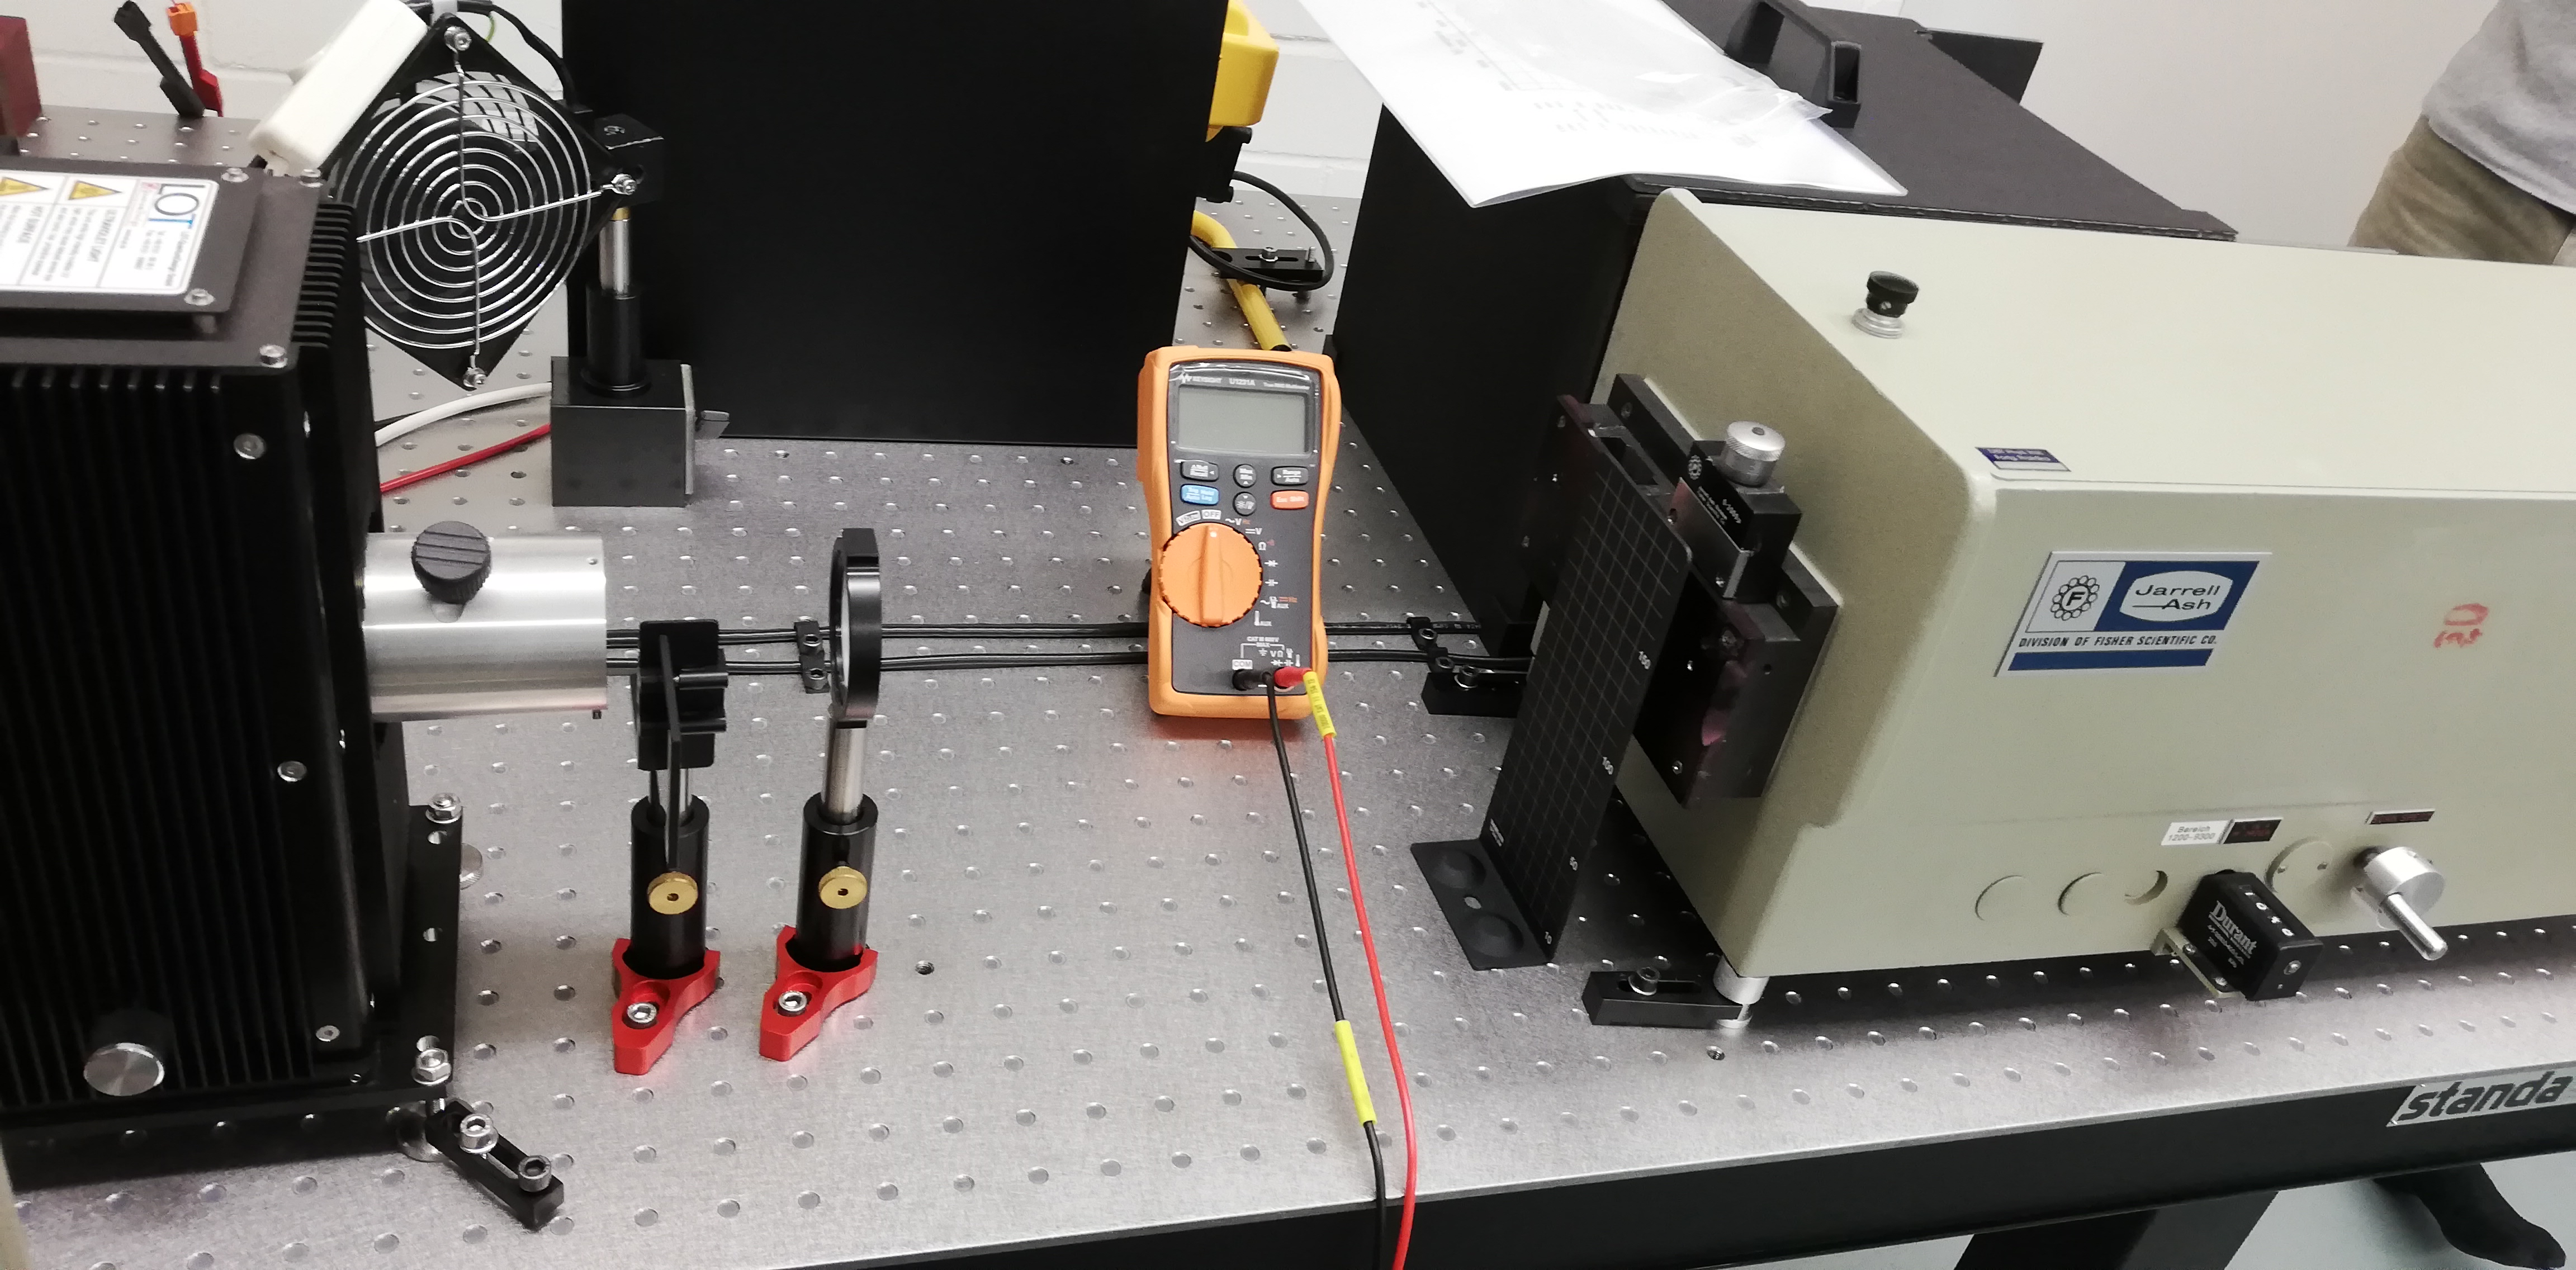
\includegraphics[width = \linewidth]{Bilder/Aufbau6.jpg}
    \caption{Xenon-Lampe mit vorgelagertem Filter}
\end{figure}

\begin{figure}[h]
    \centering
    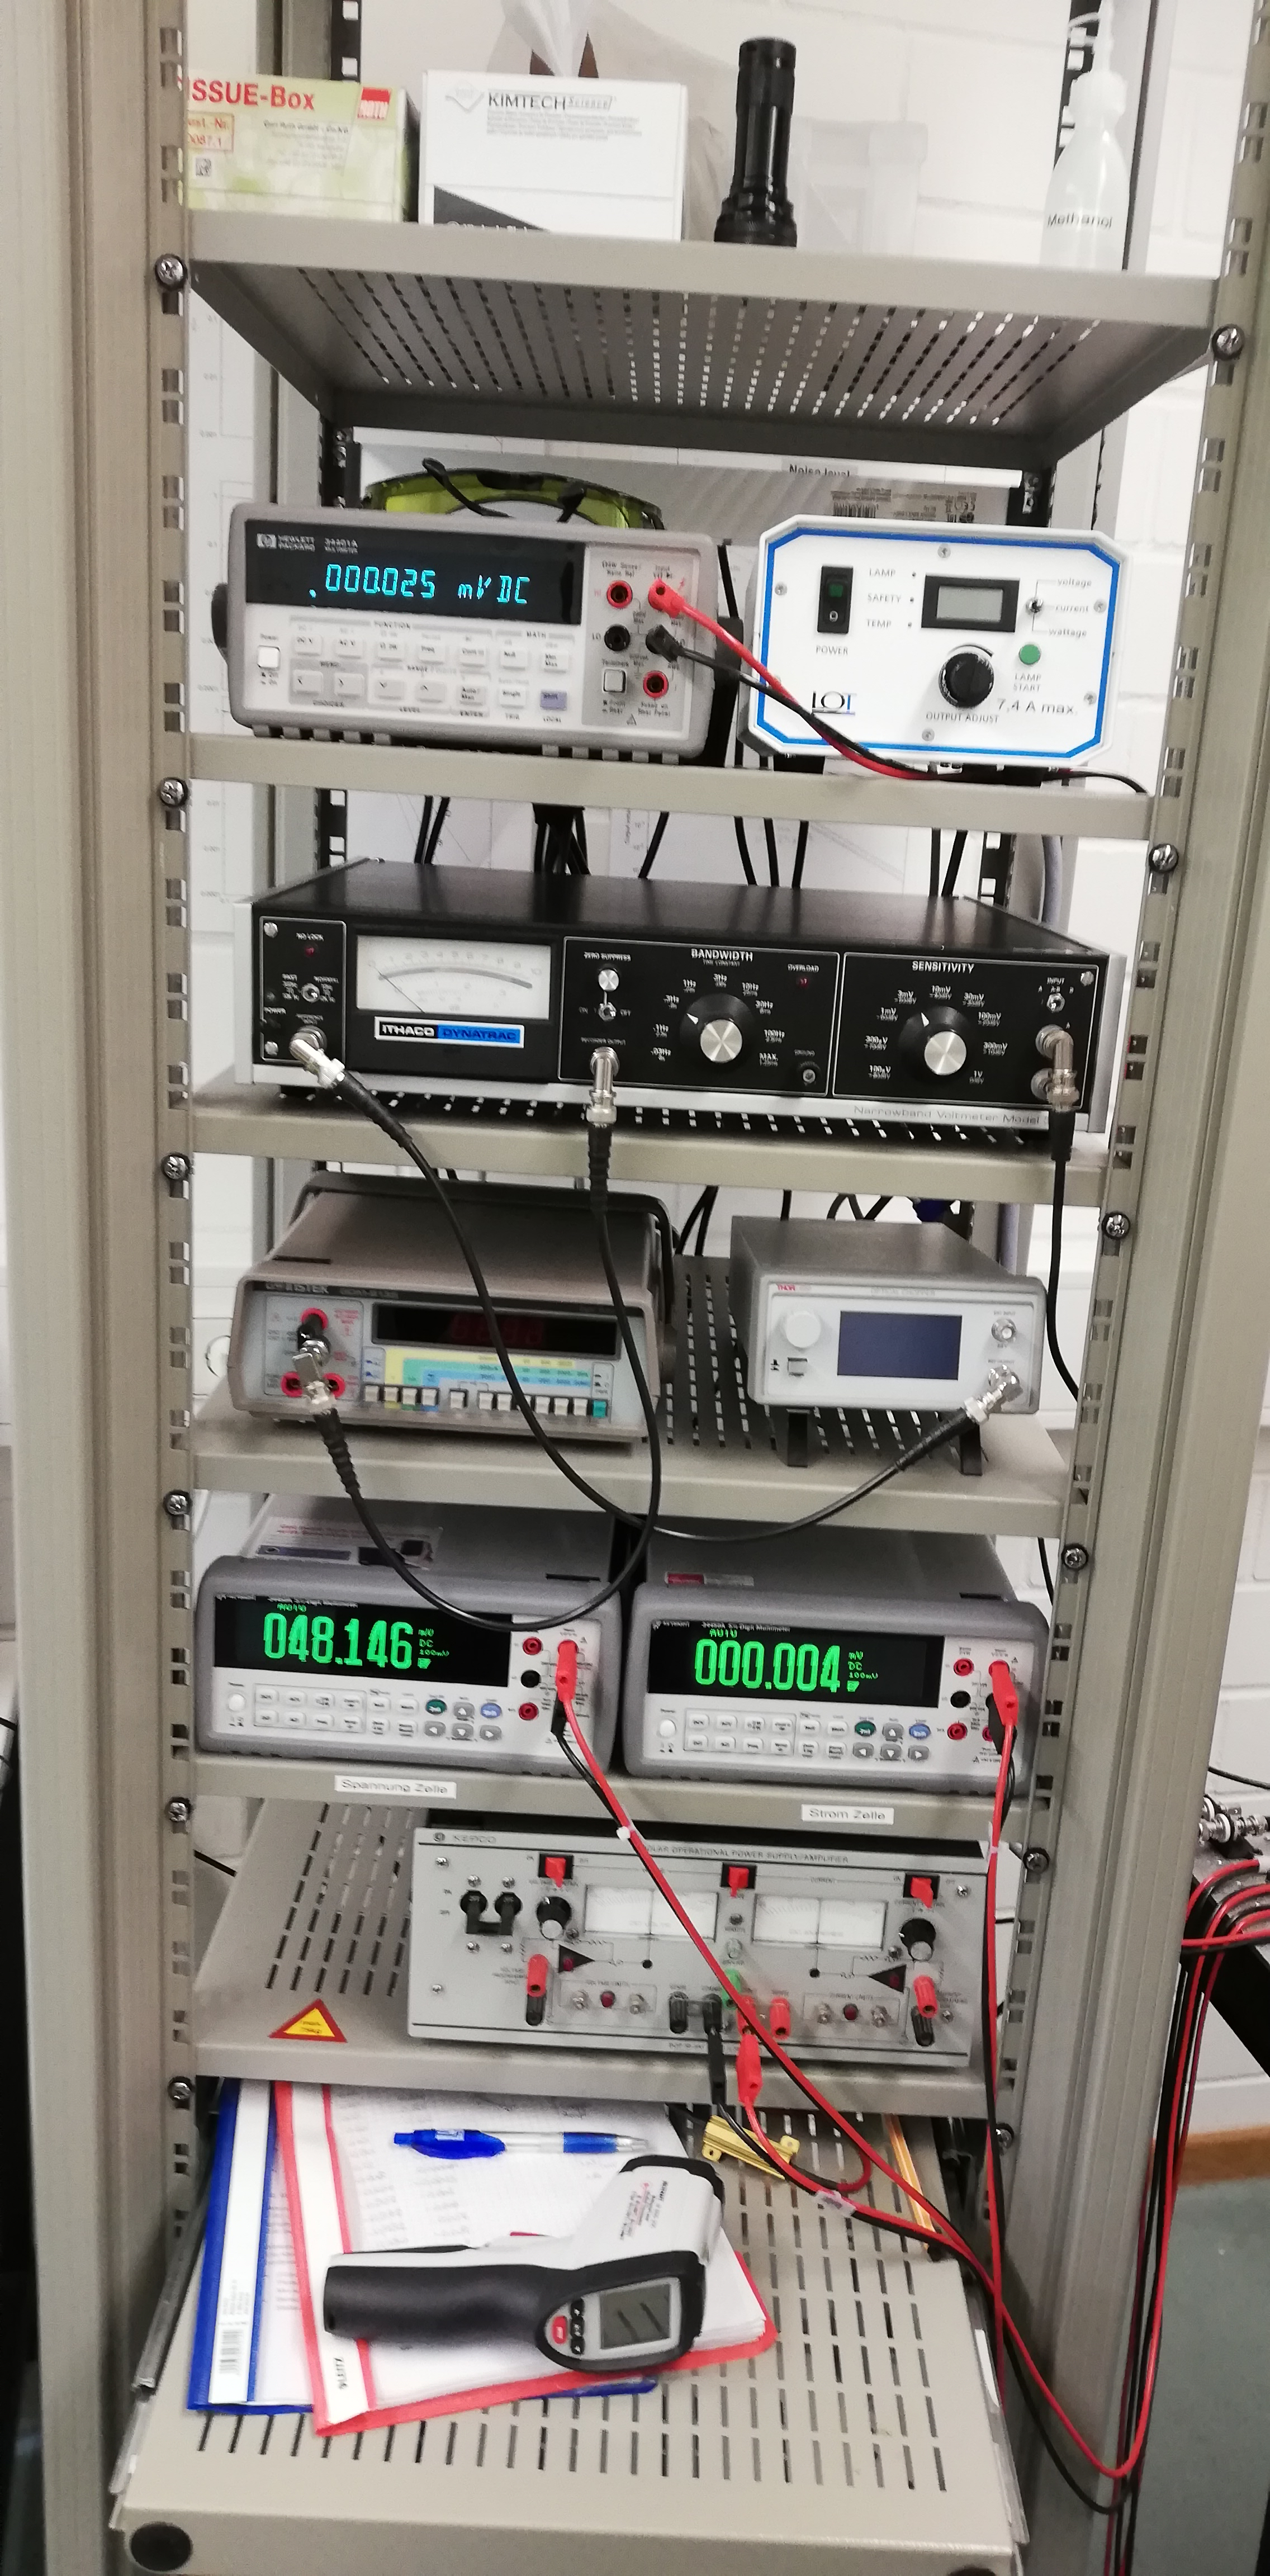
\includegraphics[width = 8cm]{Bilder/Aufbau3.jpg}
    \caption{Verwendete Messgeräte (in schwarz der Lock-in Verstärker)}
\end{figure}

\begin{figure}[h]
    \centering
    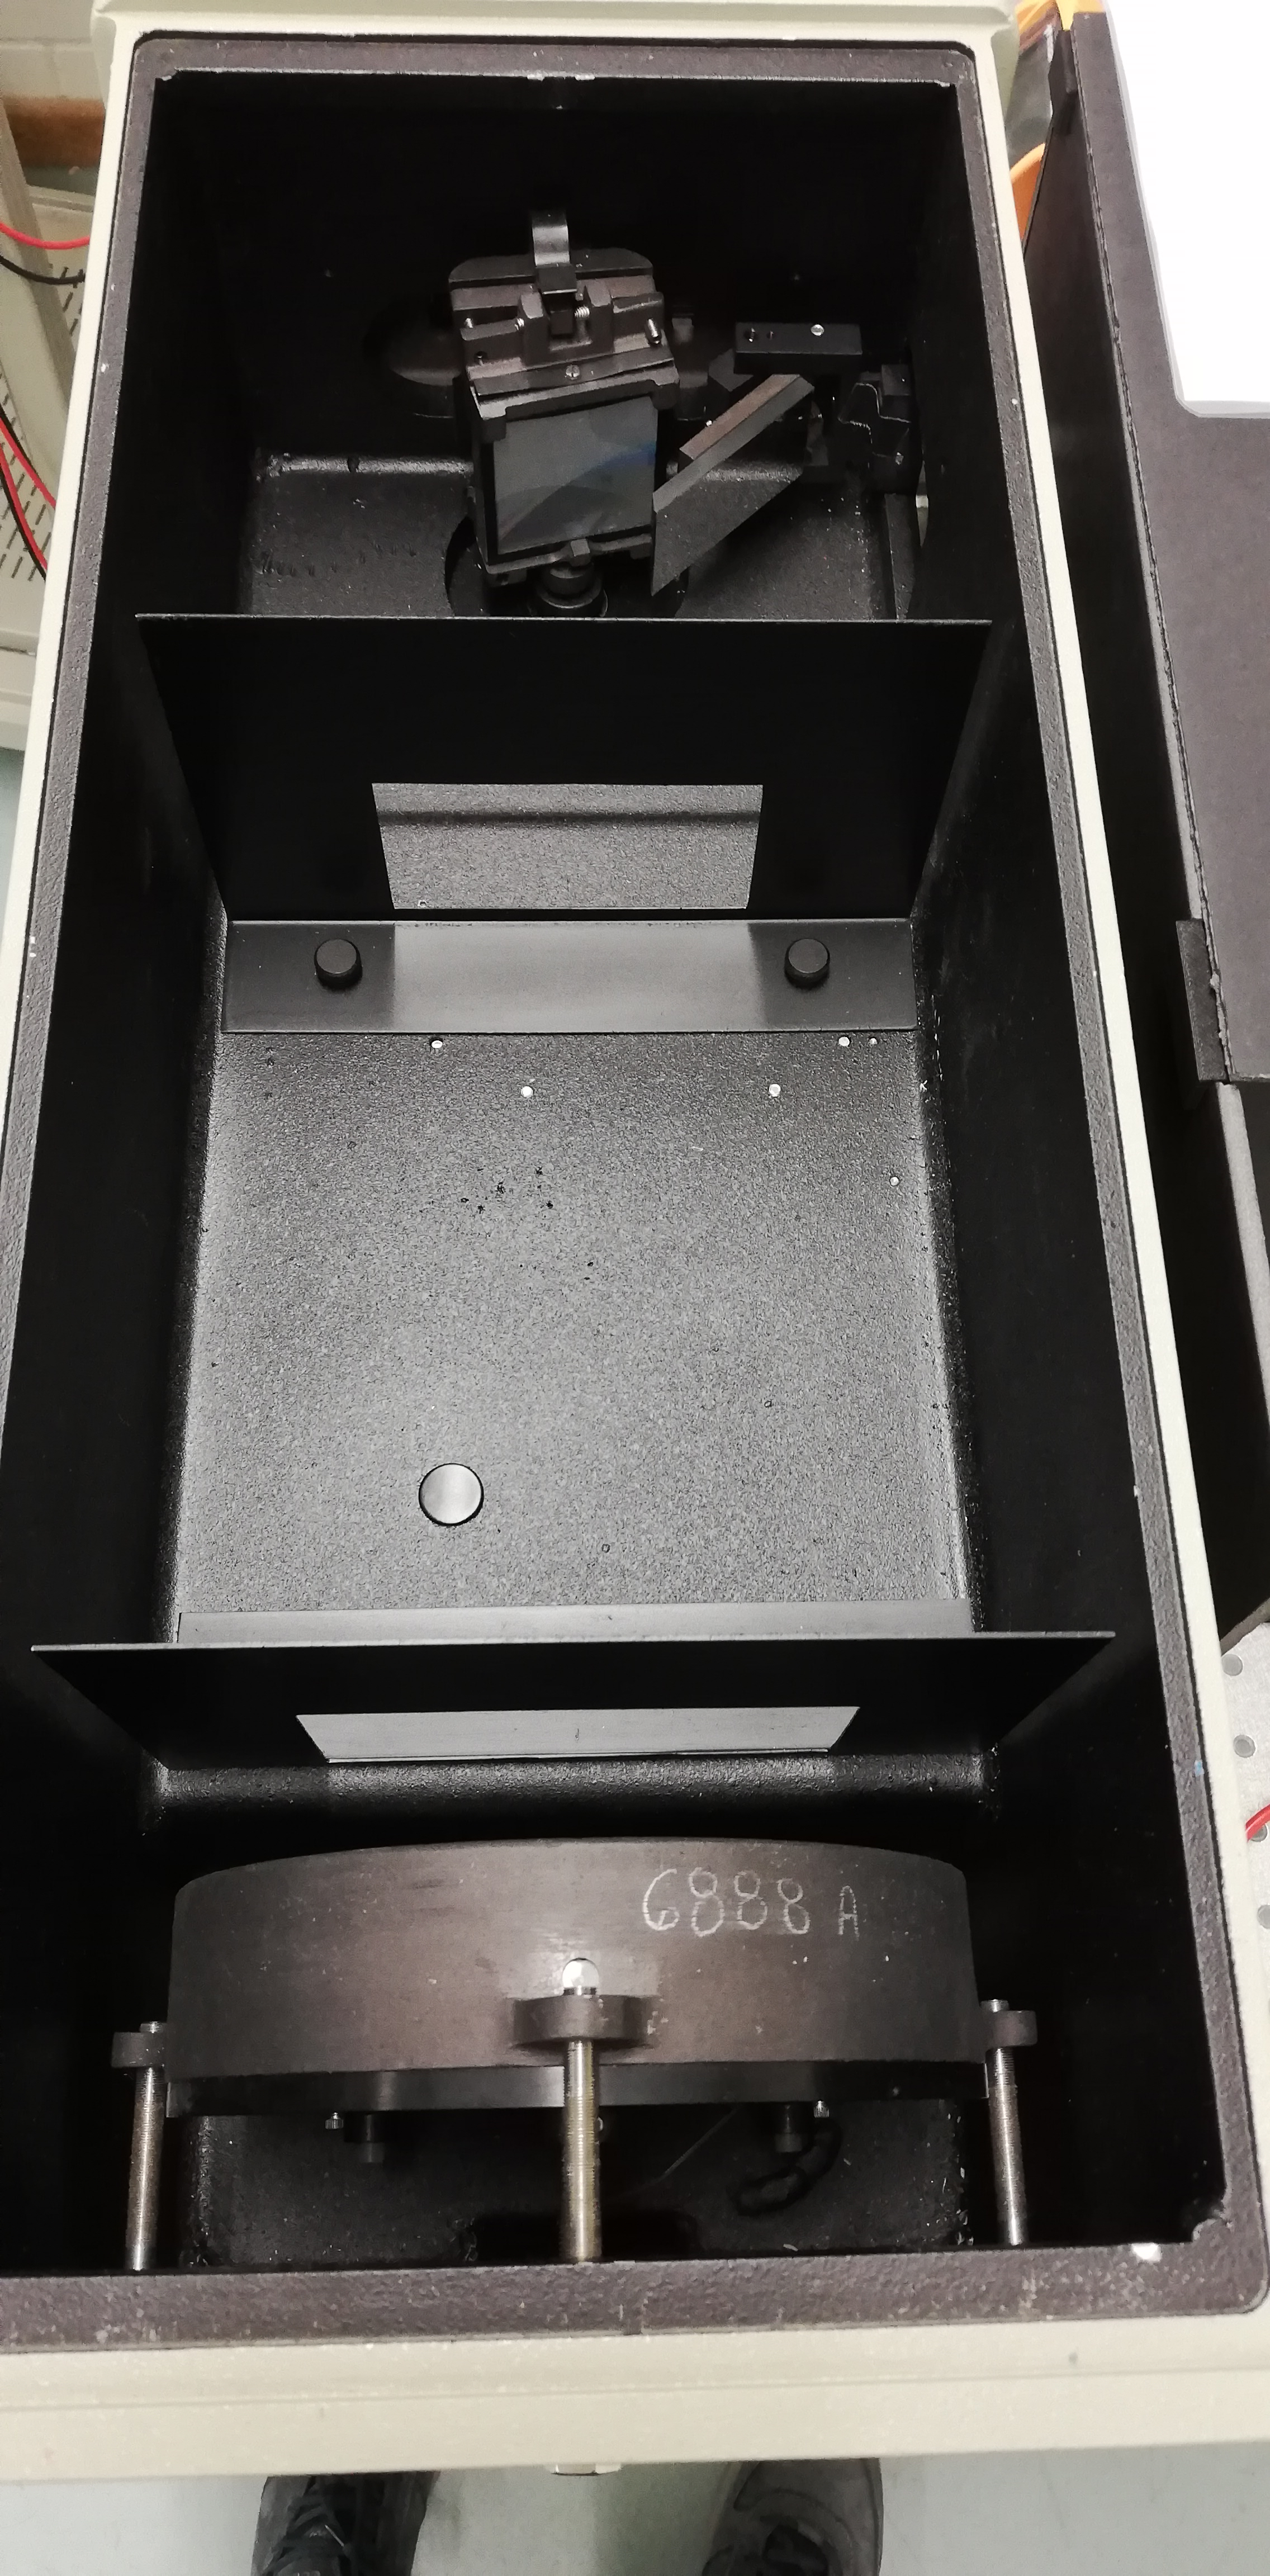
\includegraphics[width = 8cm]{Bilder/Aufbau4.jpg}
    \caption{Innenansicht des Gitterspektrometers}
\end{figure}
\clearpage


\subsubsection{Versuchsteil U-I-Kennlinien}

\begin{figure}[h]
    \centering
    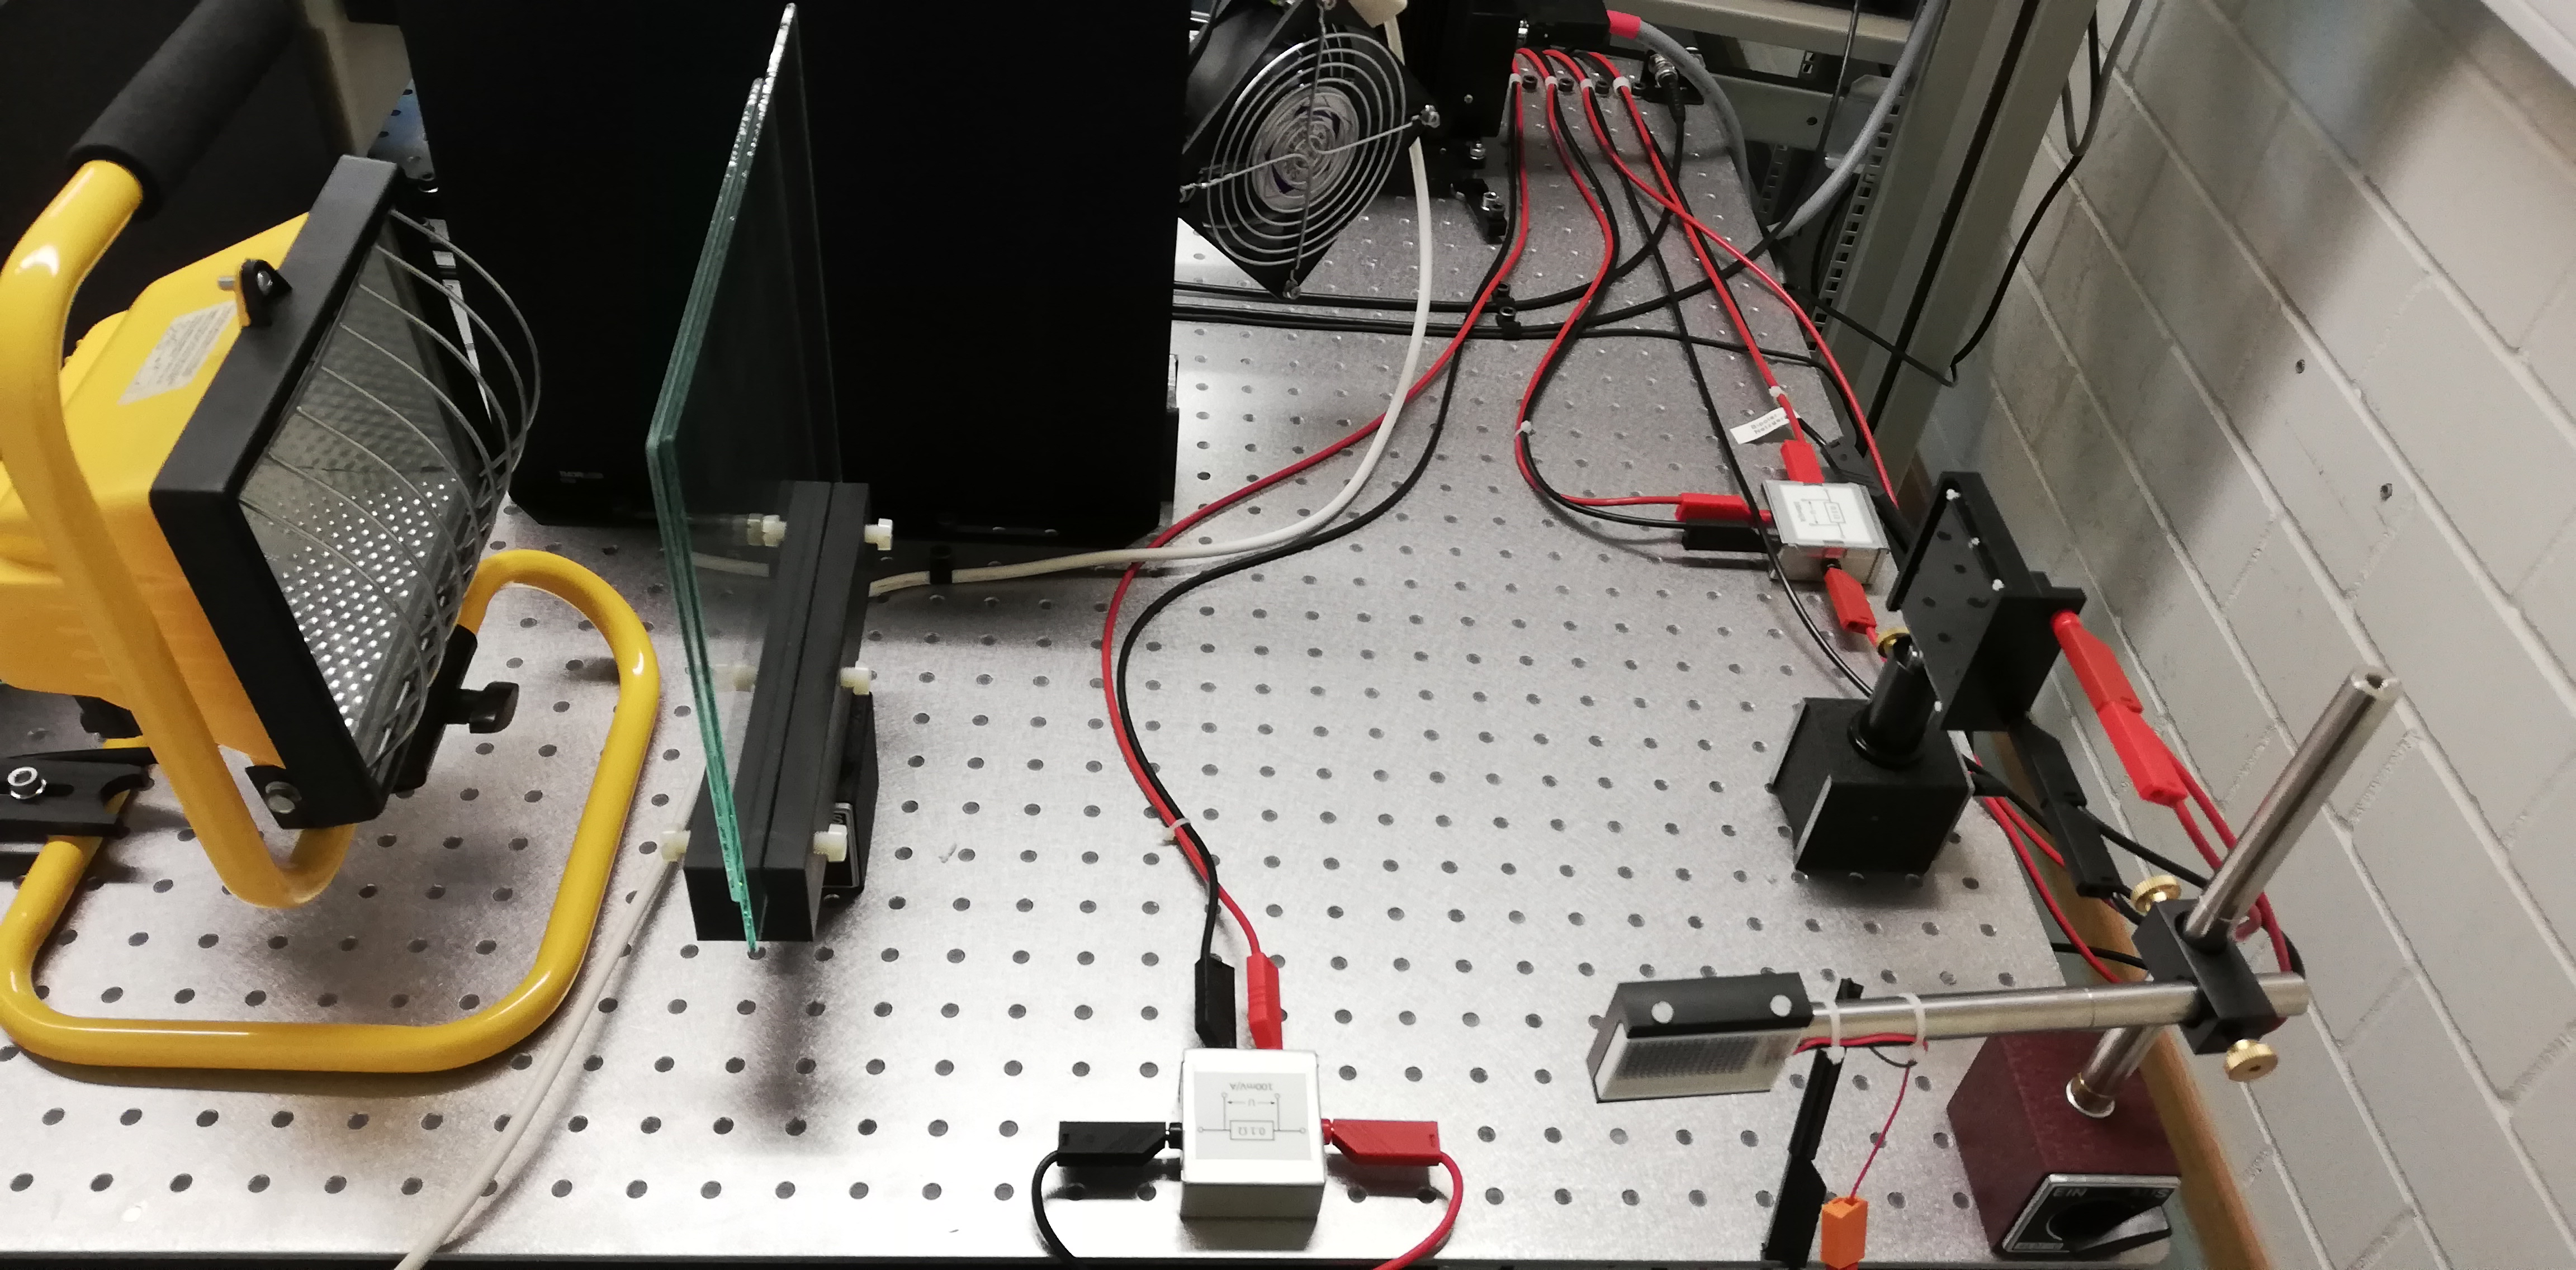
\includegraphics[width = \linewidth]{Bilder/Aufbau1.jpg}
    \caption{Baustrahler mit vorgelagerten Glasplatten}
\end{figure}


\clearpage
\subsection{Messdaten}

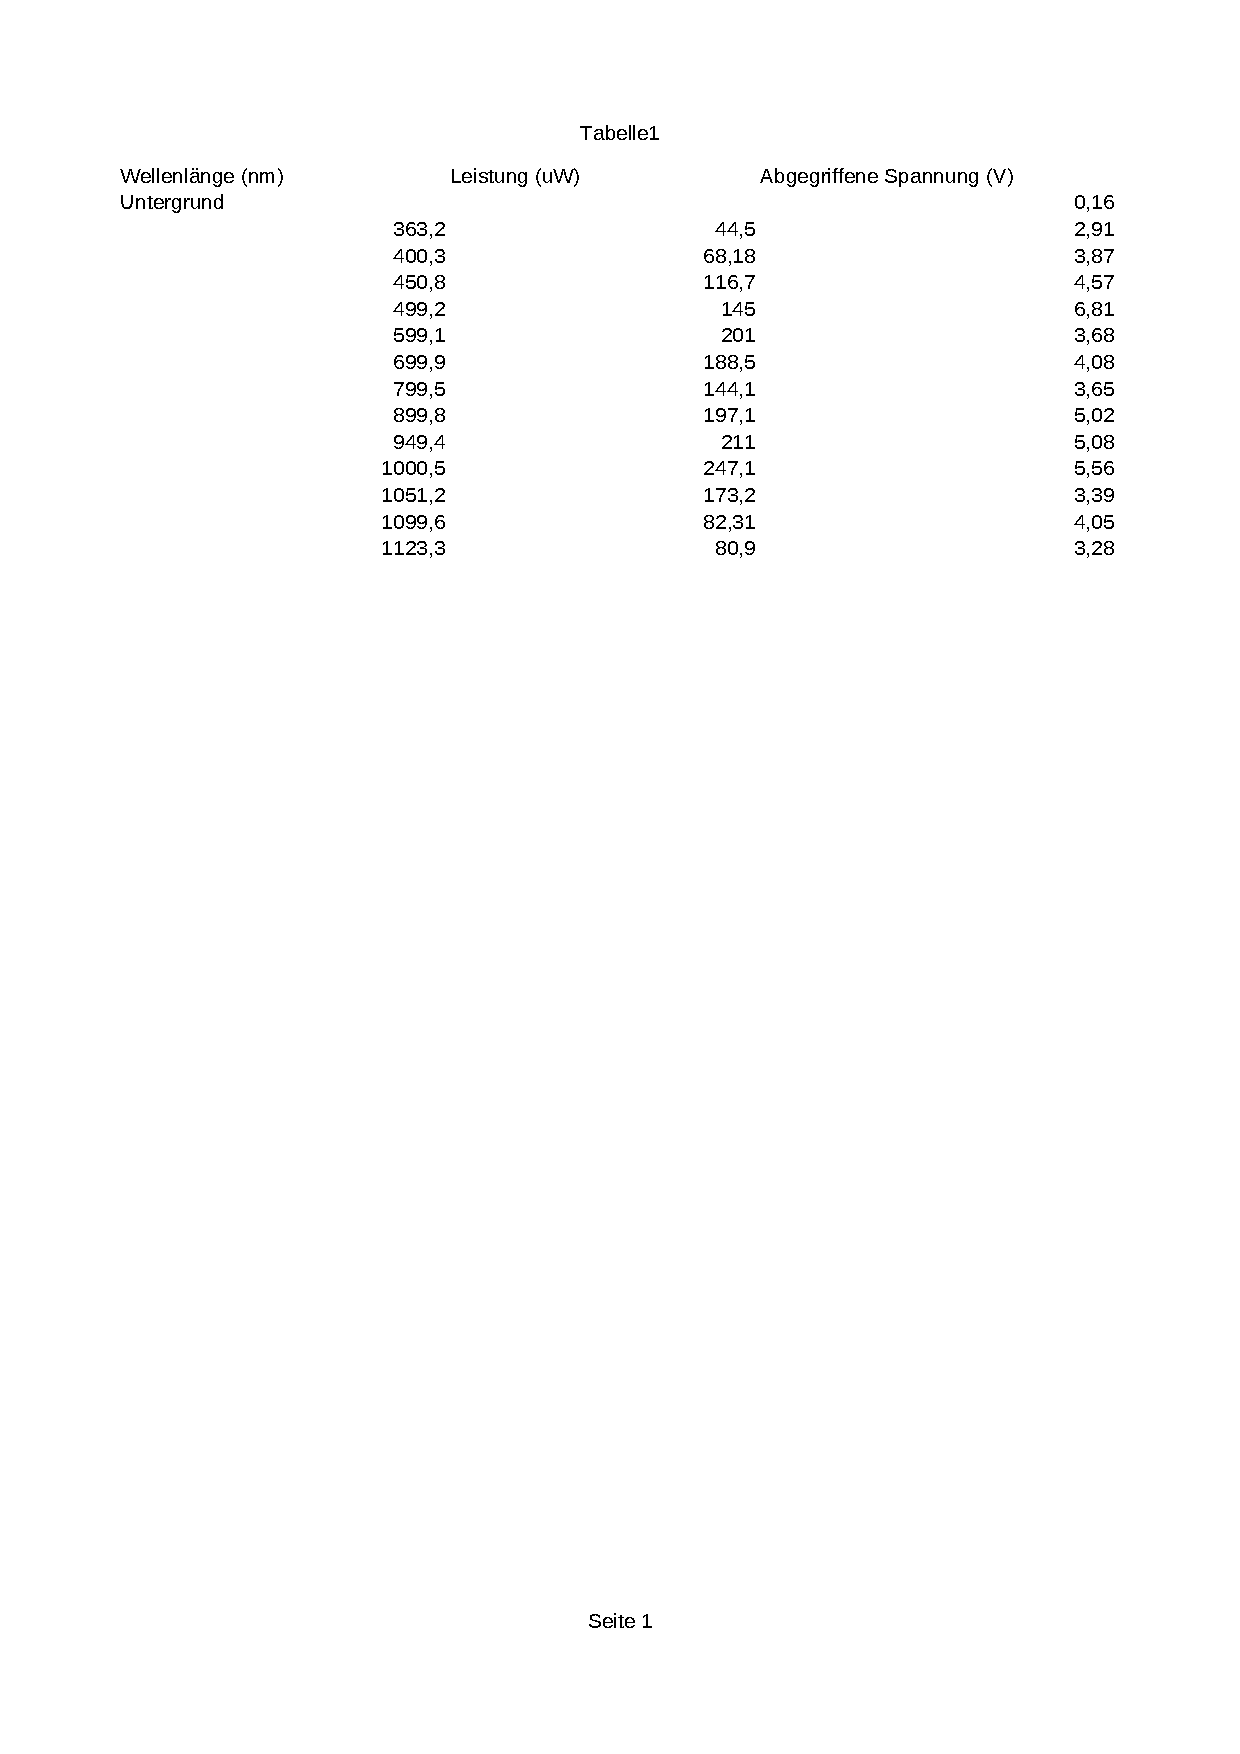
\includepdf[pages=-]{Messwerte/Messung32CIS.pdf}
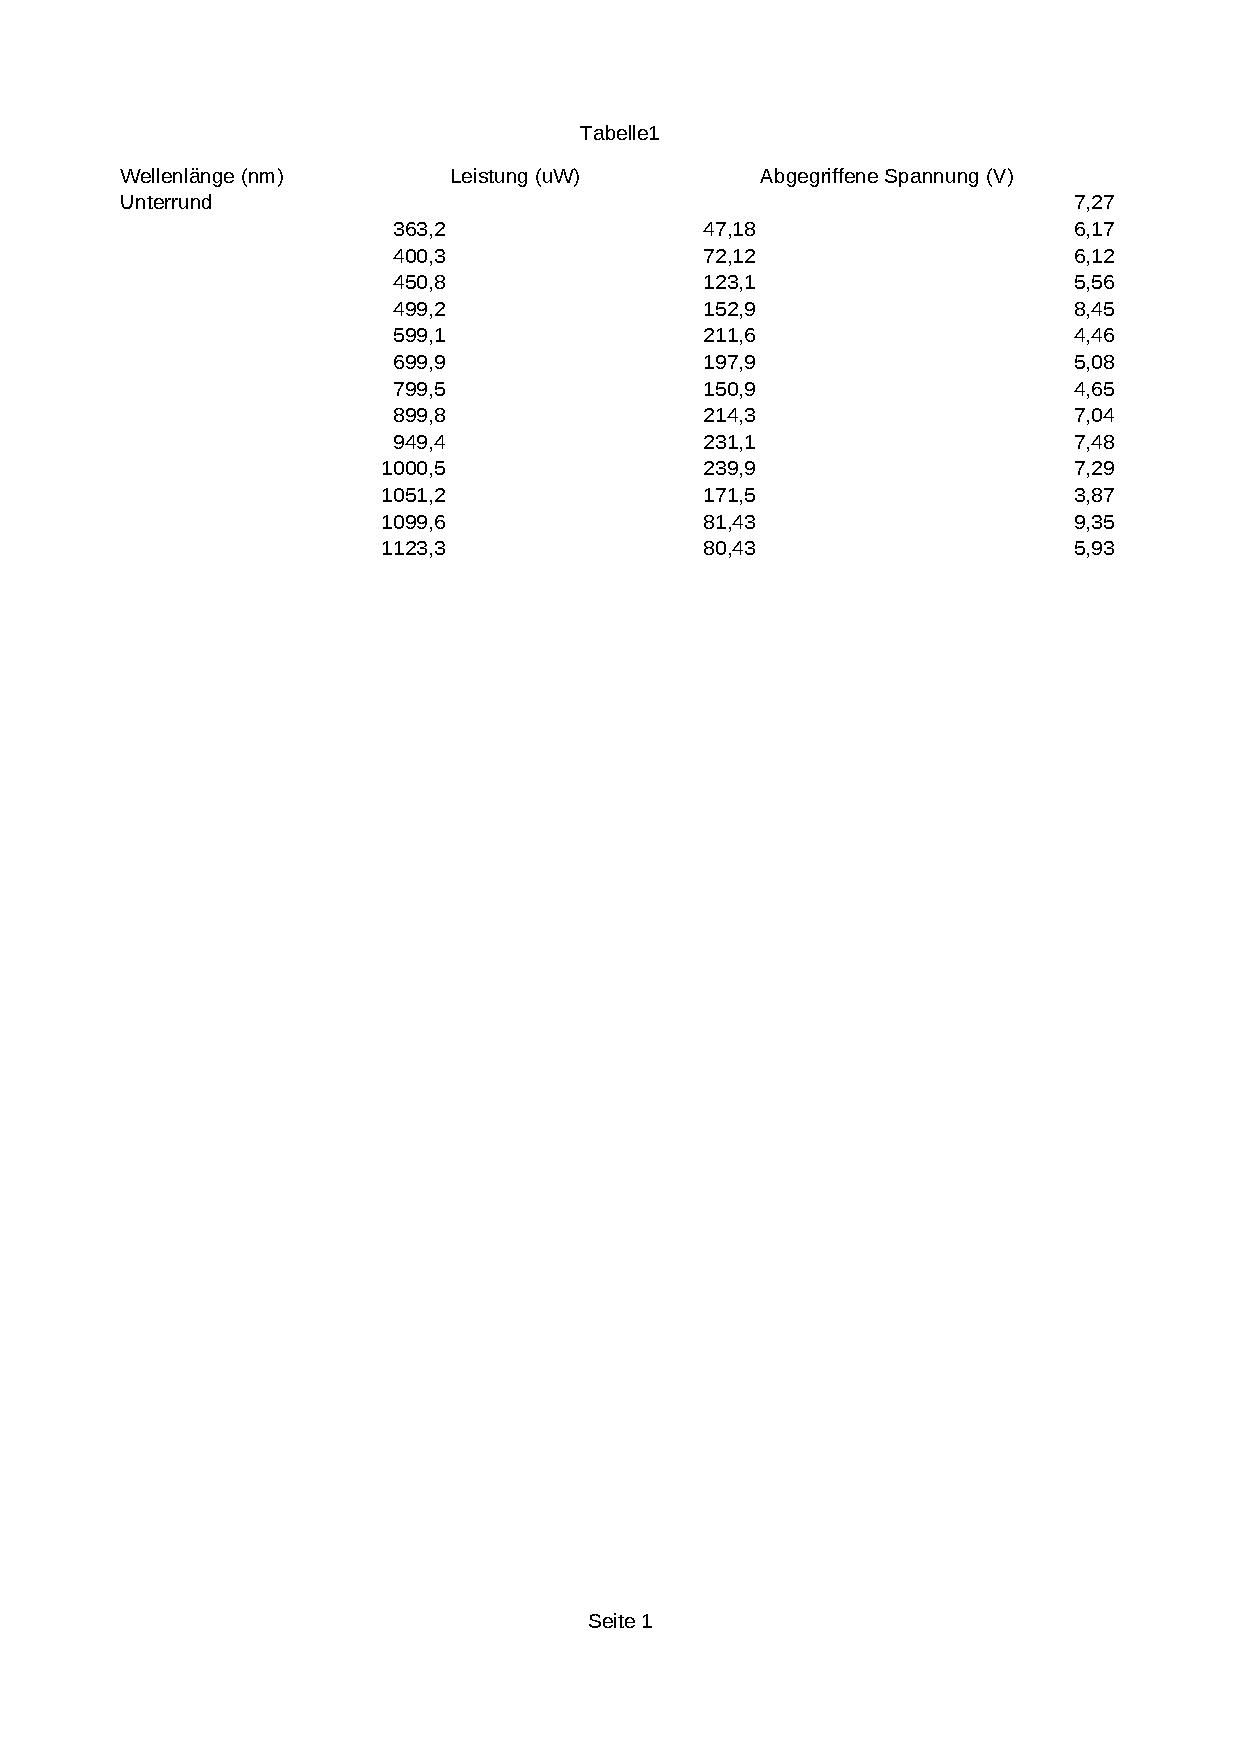
\includepdf[pages=-]{Messwerte/Messung32Monokristallin.pdf}
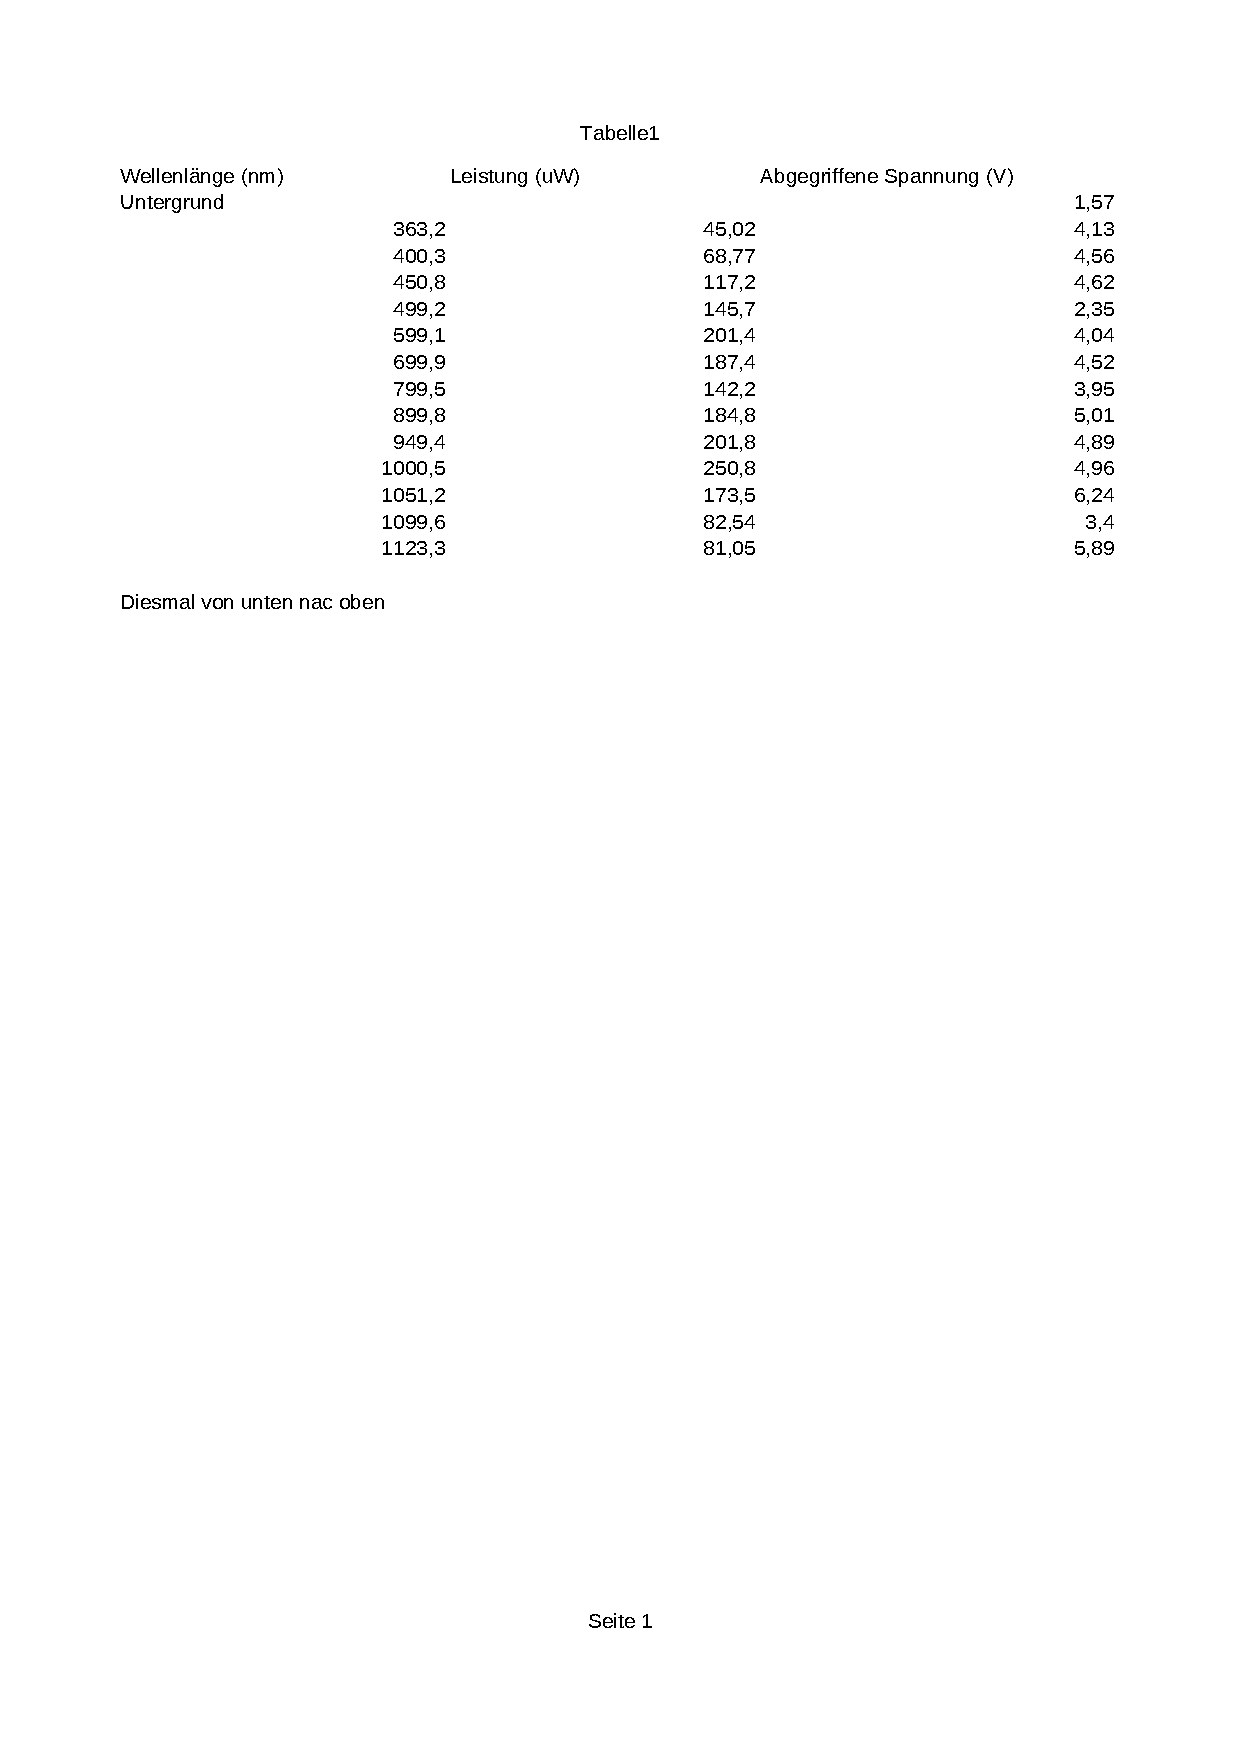
\includepdf[pages=-]{Messwerte/Messung32Multikrist.pdf}
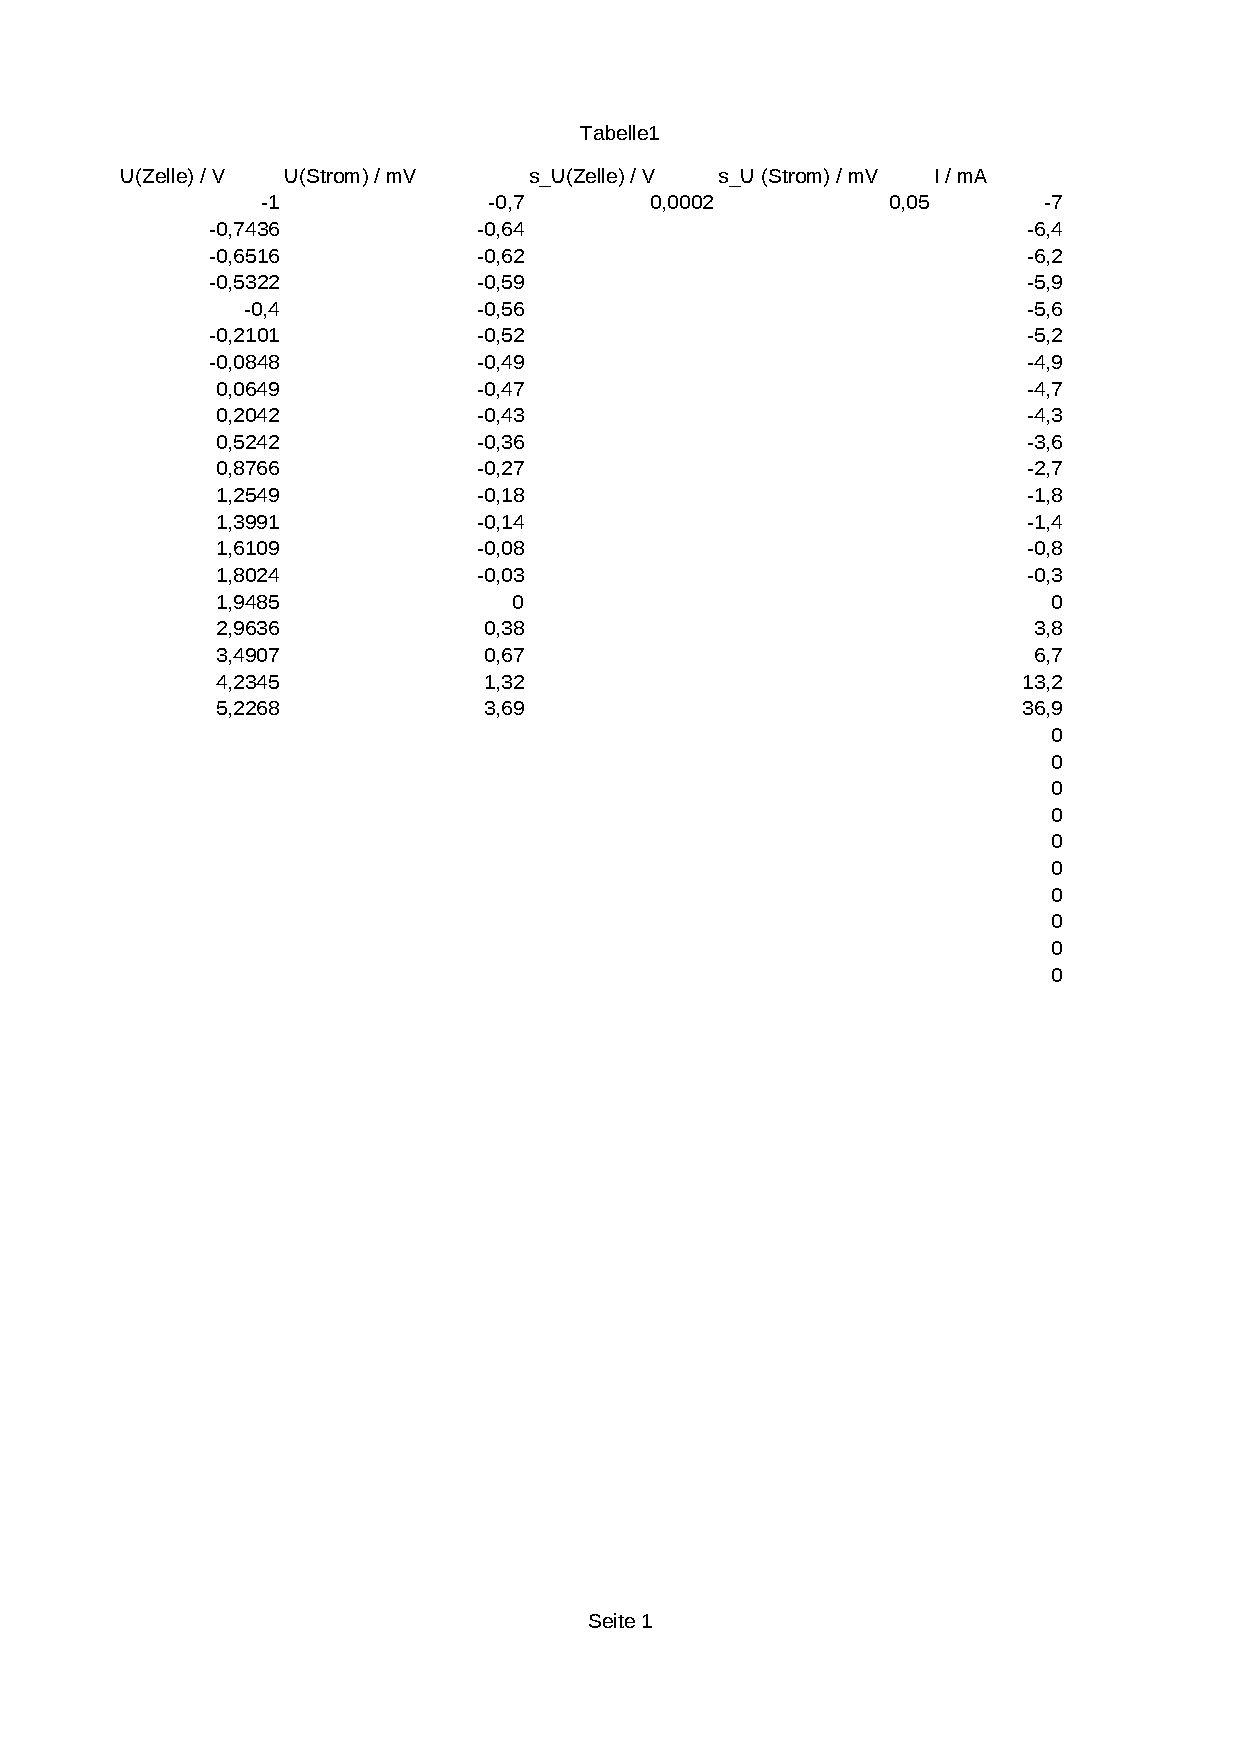
\includepdf[pages=-]{Messwerte/Messung33CIS130.pdf}
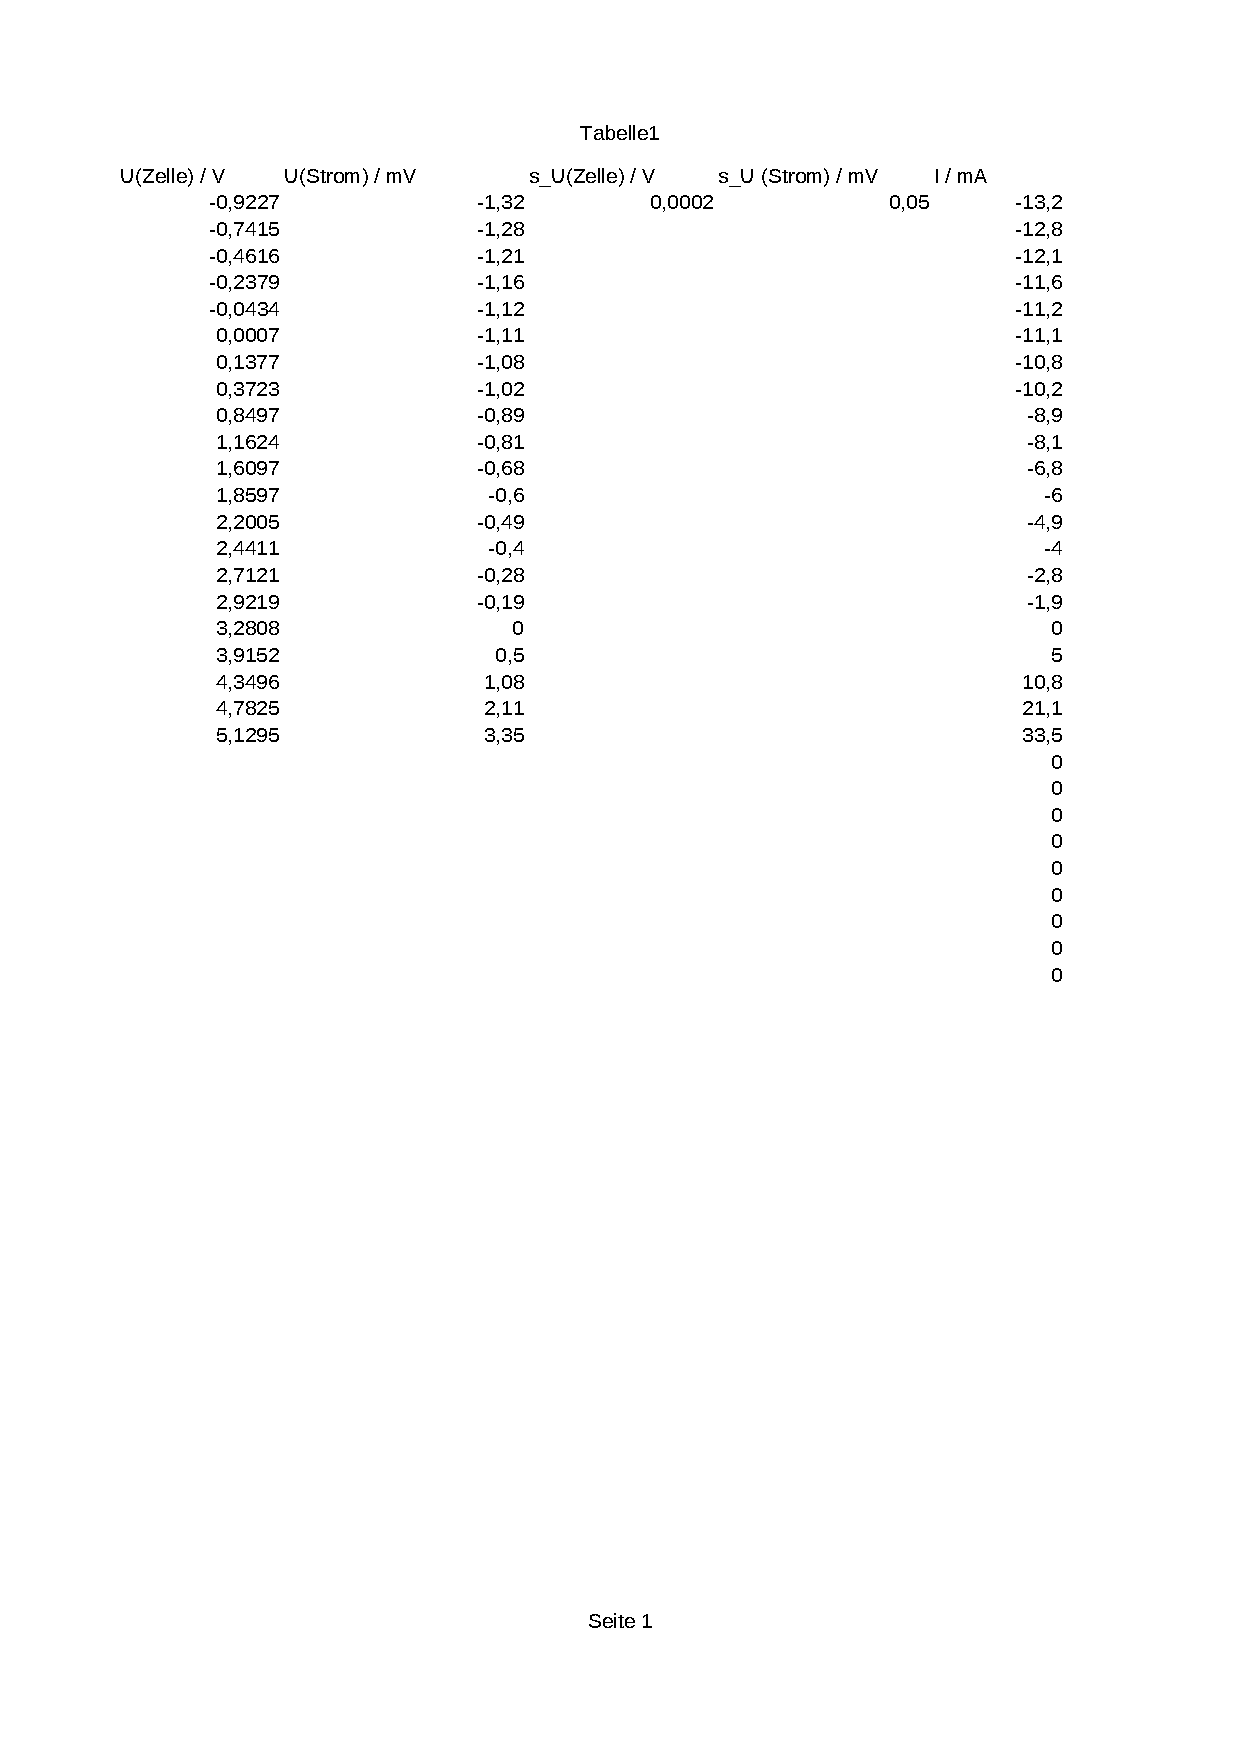
\includepdf[pages=-]{Messwerte/Messung33CIS180.pdf}
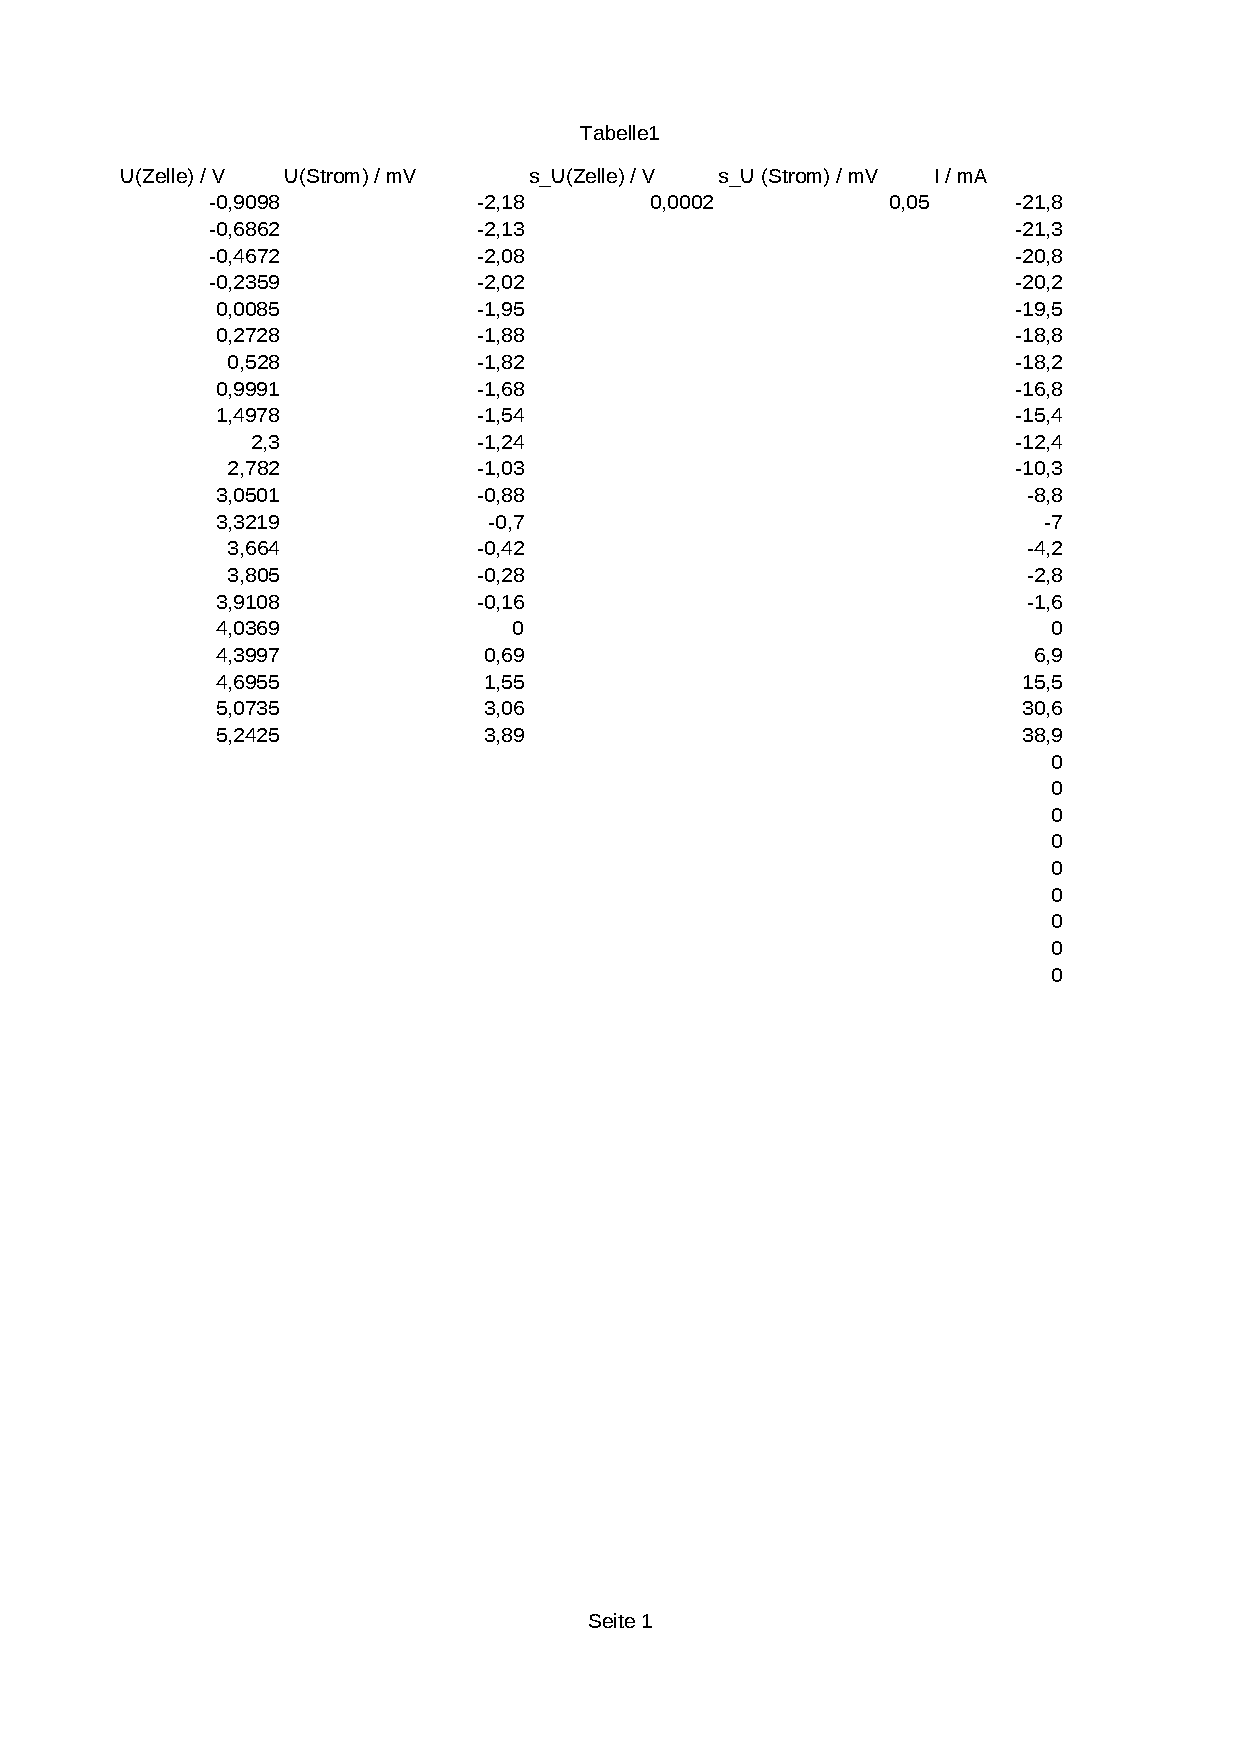
\includepdf[pages=-]{Messwerte/Messung33CIS230.pdf}
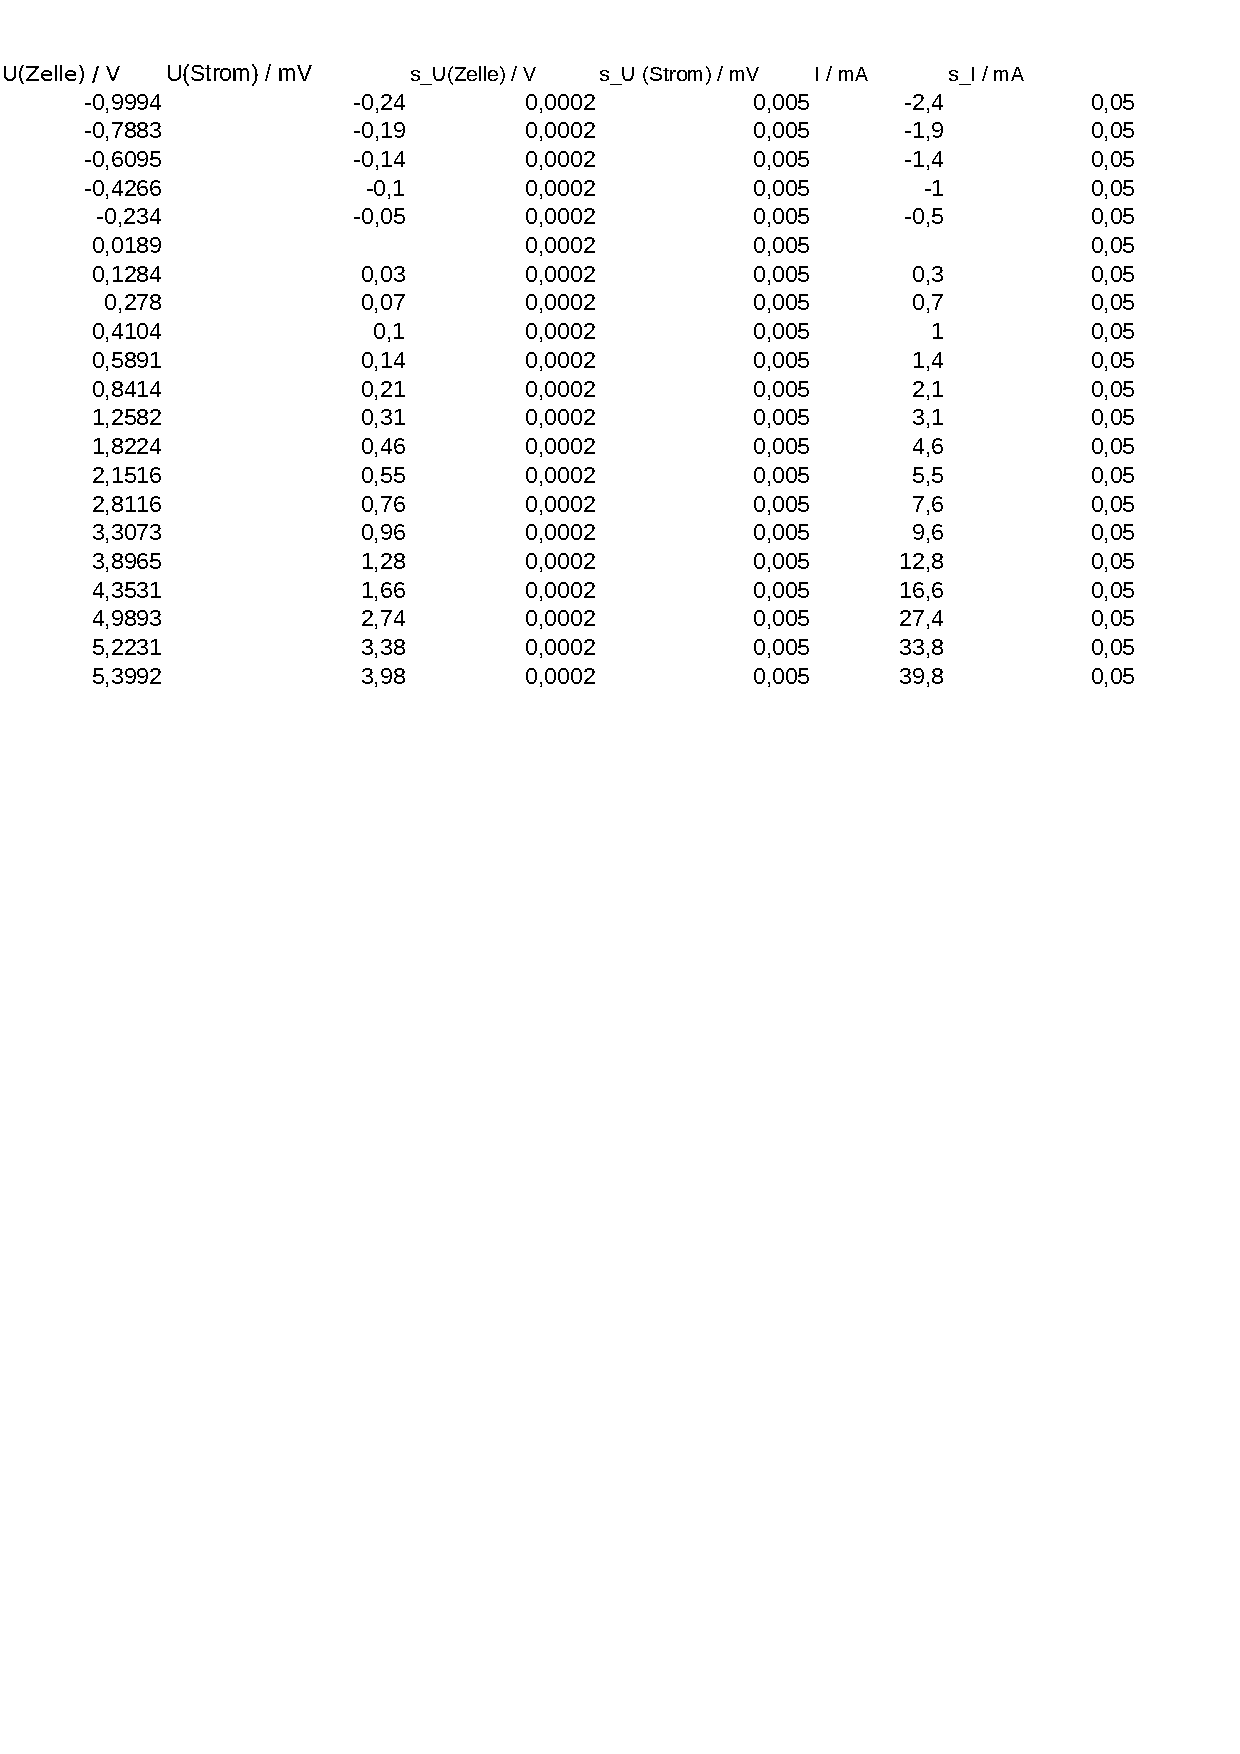
\includepdf[pages=-]{Messwerte/Messung33CISdunkel.pdf}
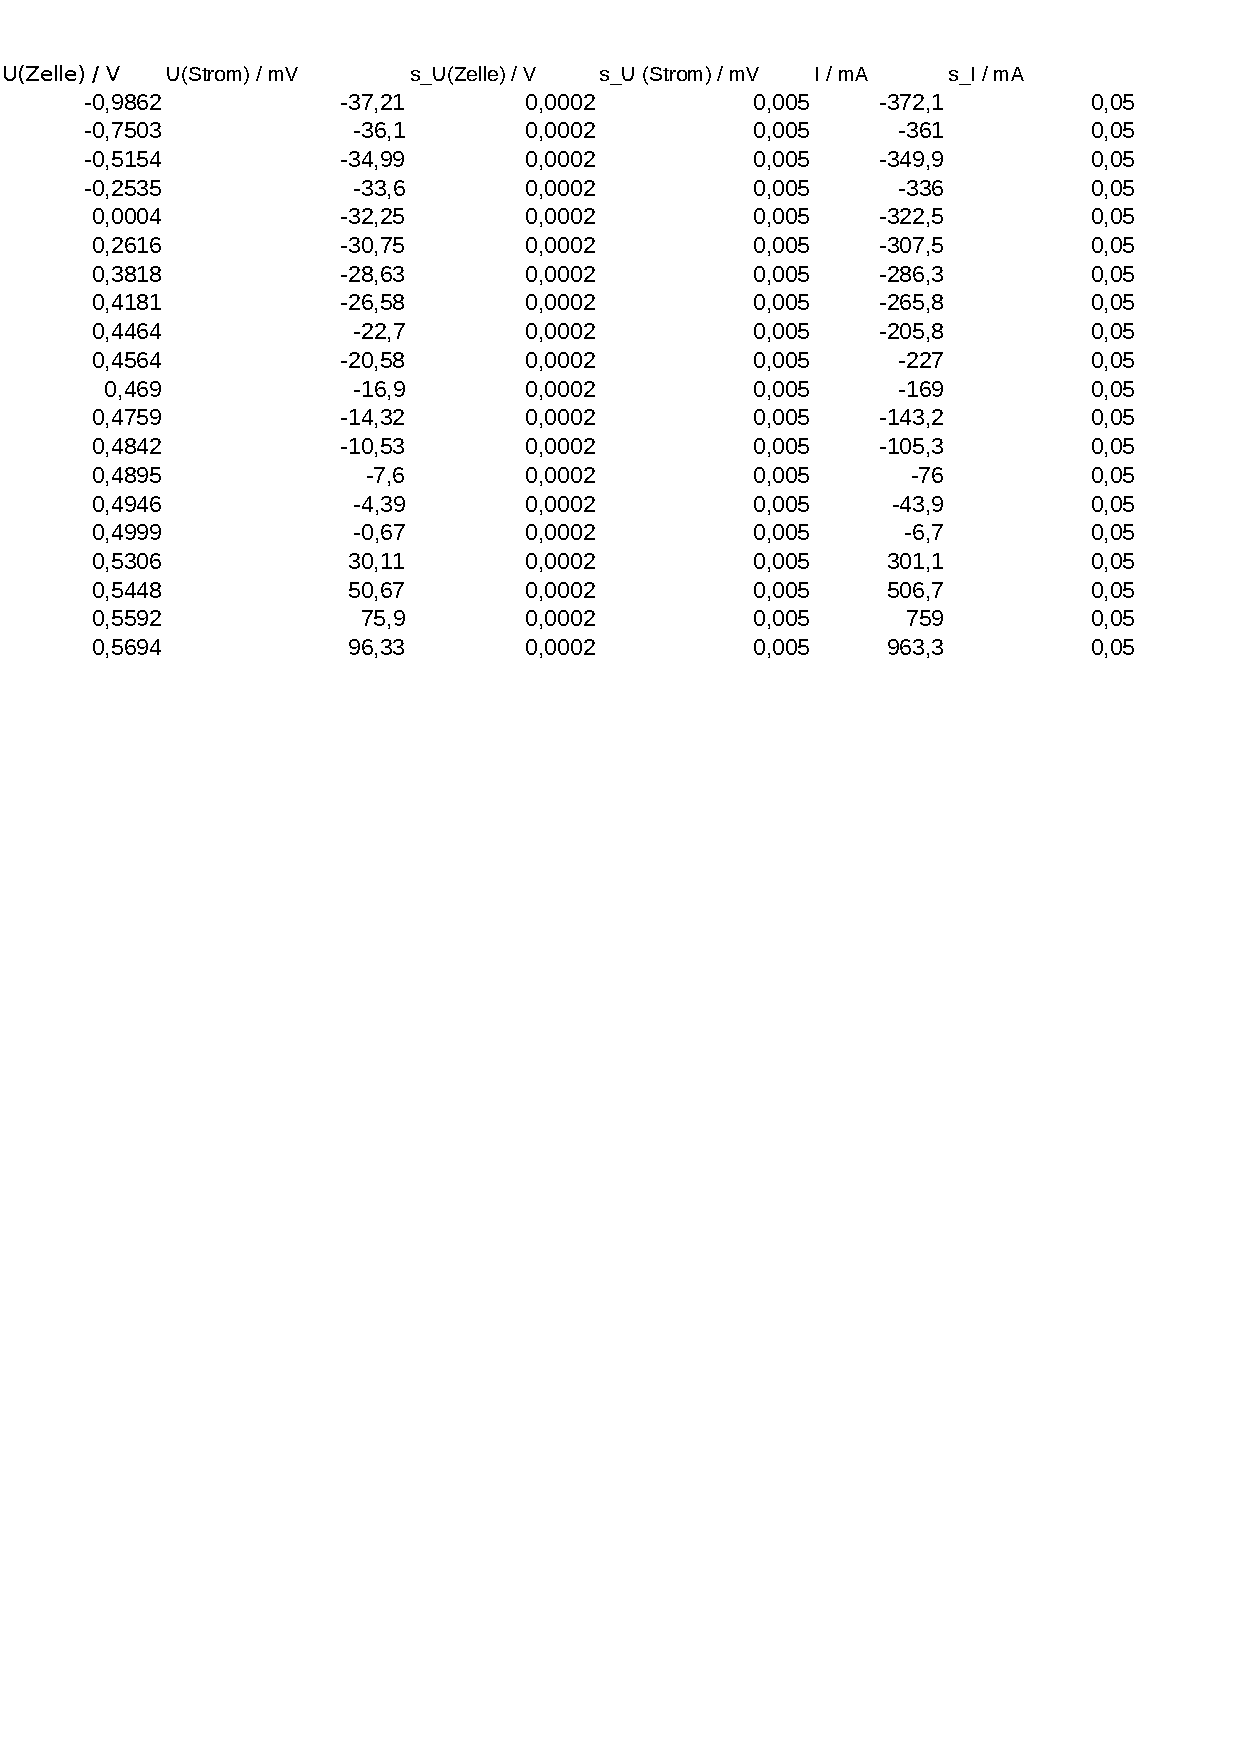
\includepdf[pages=-]{Messwerte/Messung33SiMono130.pdf}
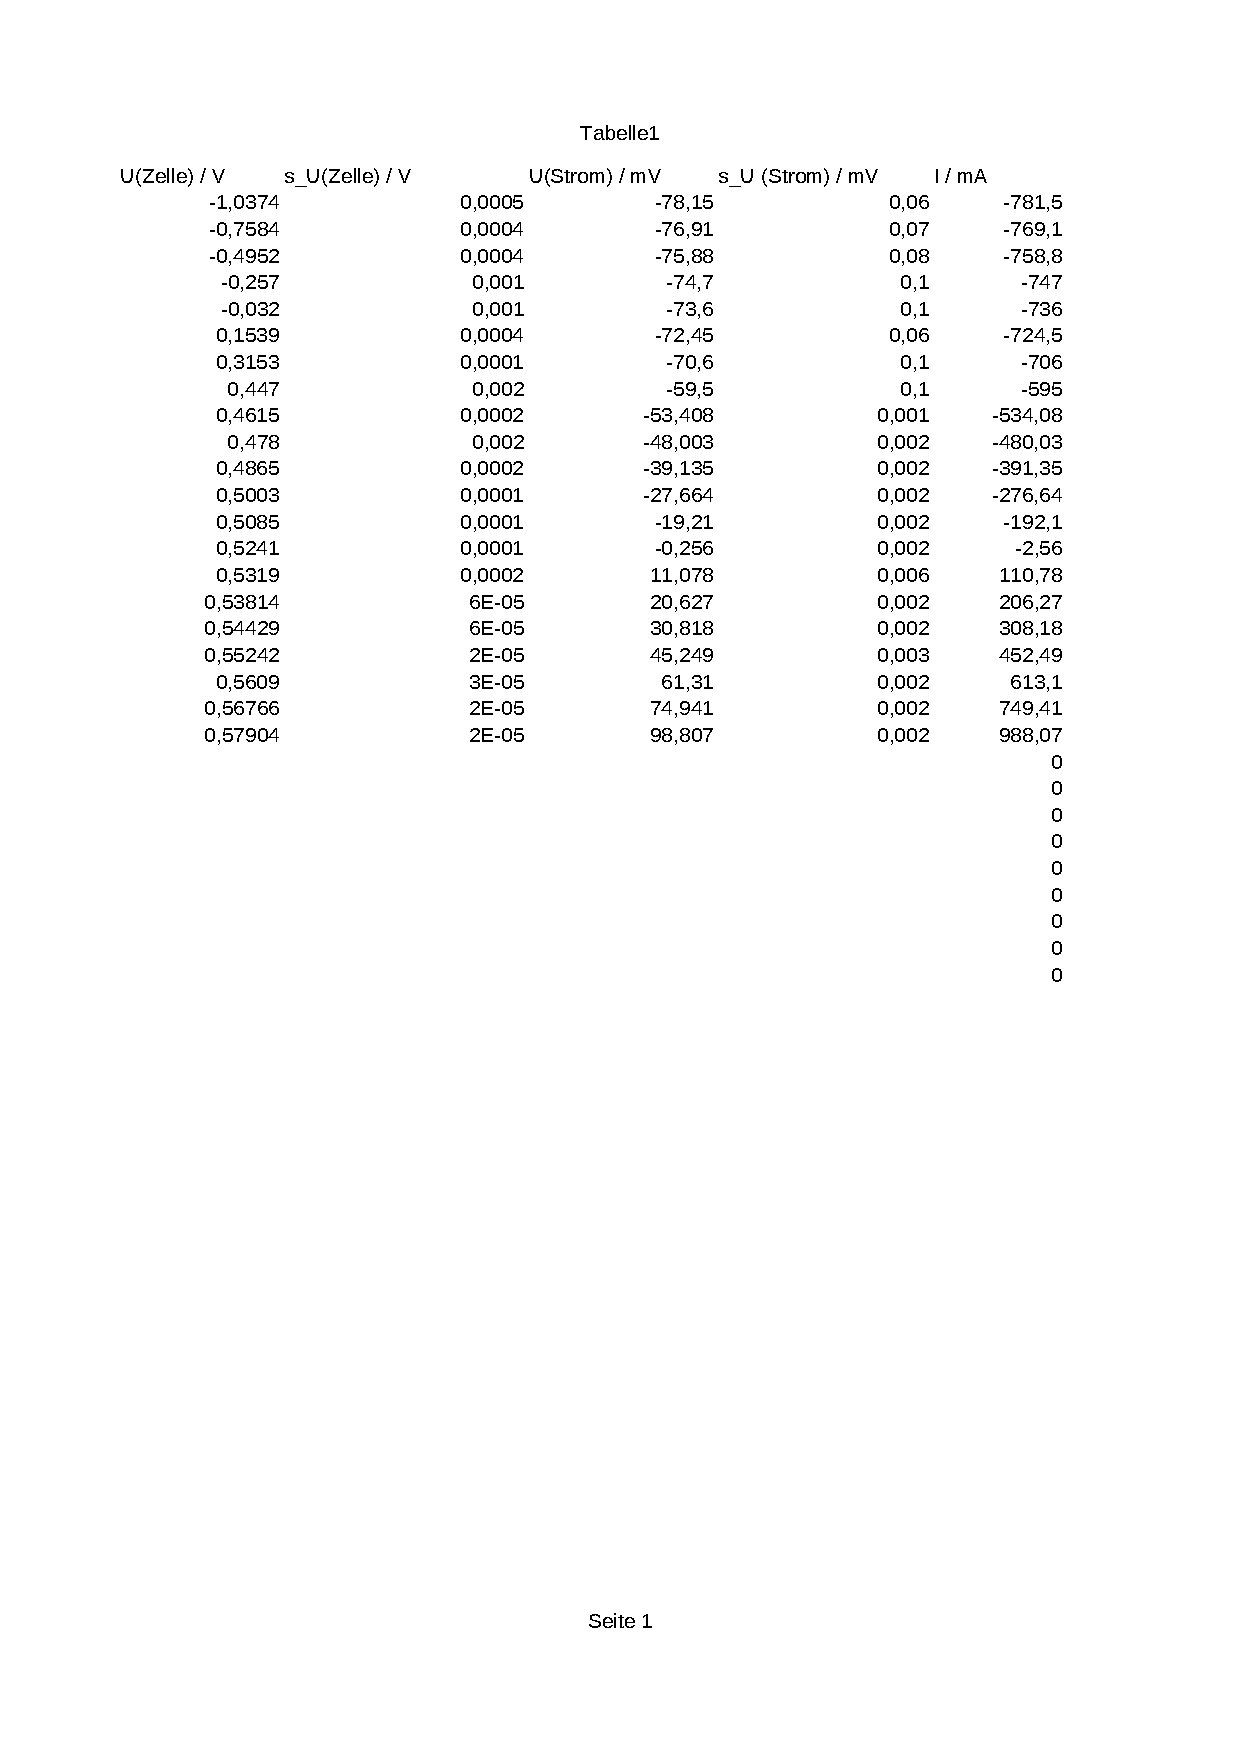
\includepdf[pages=-]{Messwerte/Messung33SiMono180.pdf}
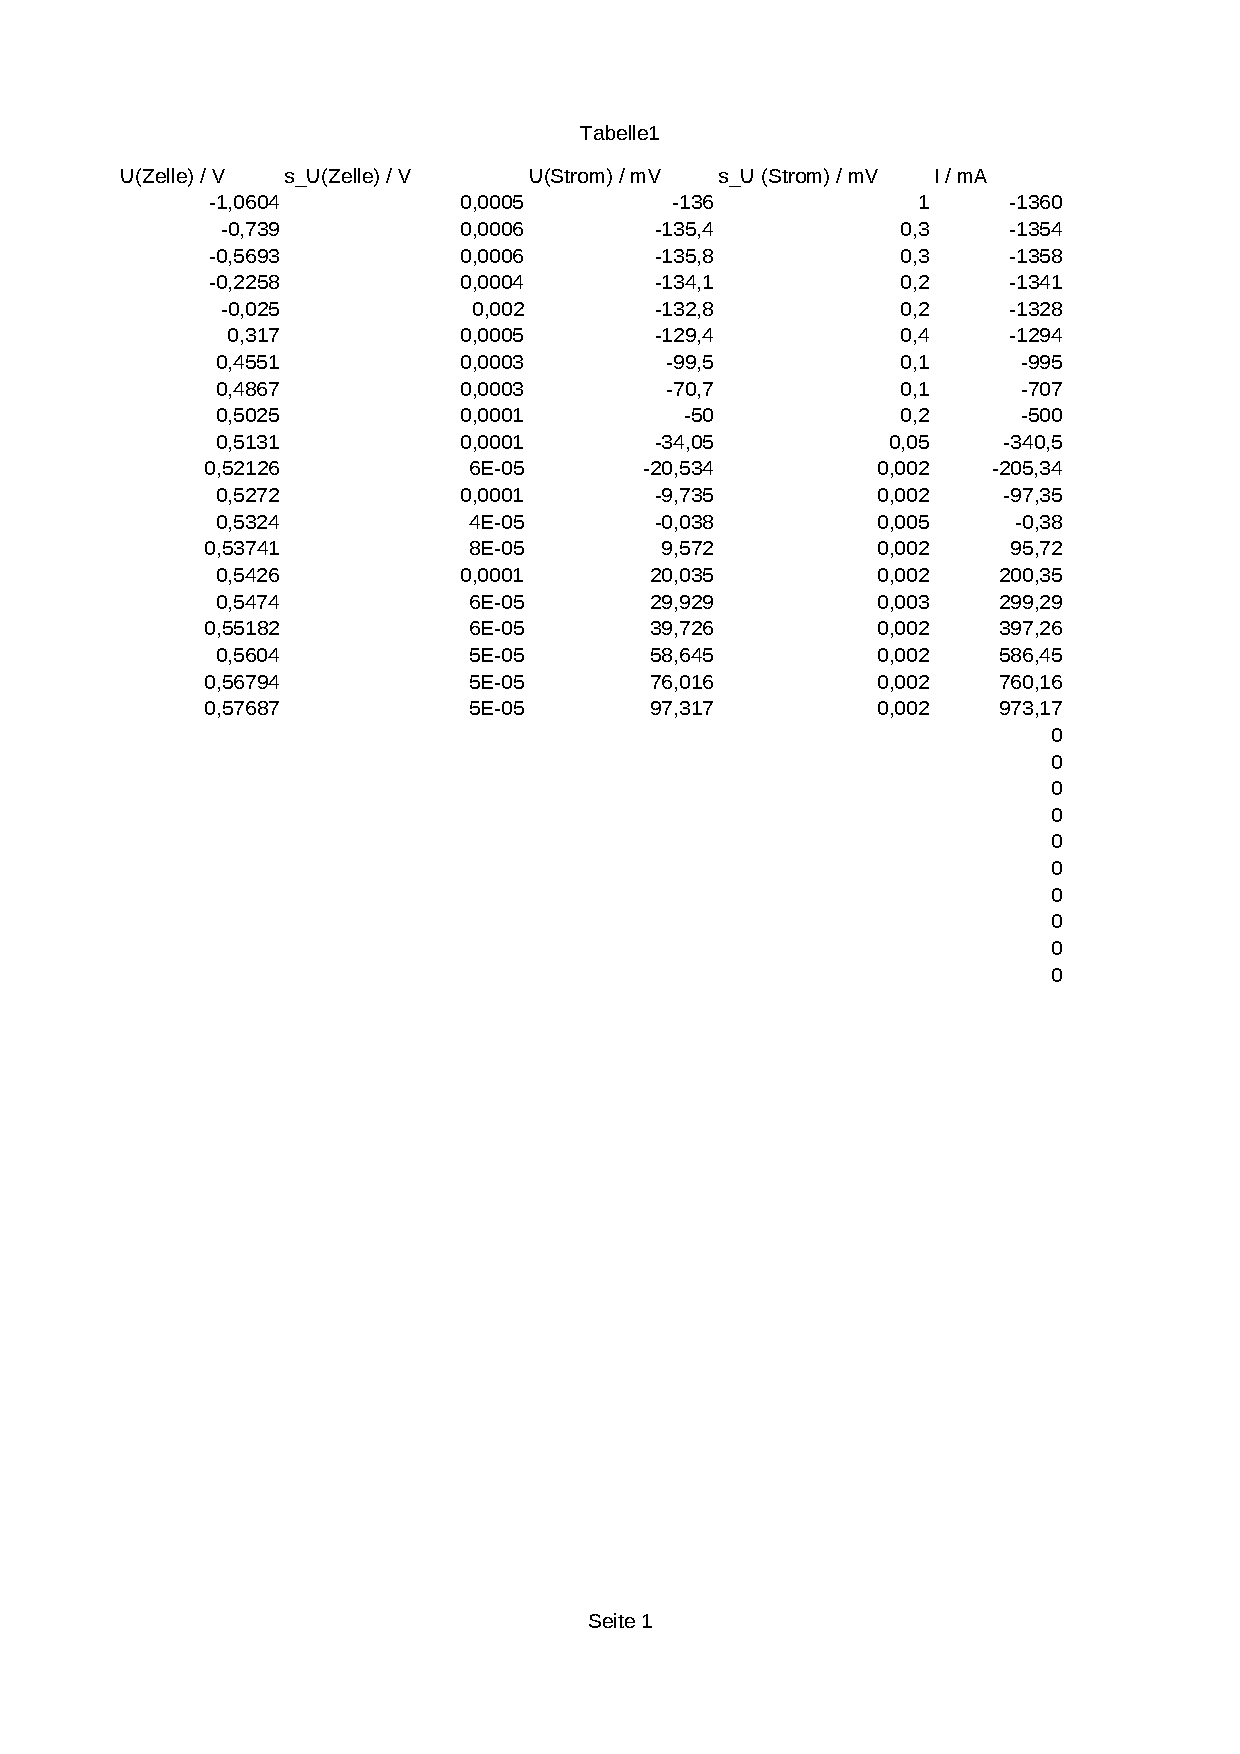
\includepdf[pages=-]{Messwerte/Messung33SiMono230.pdf}
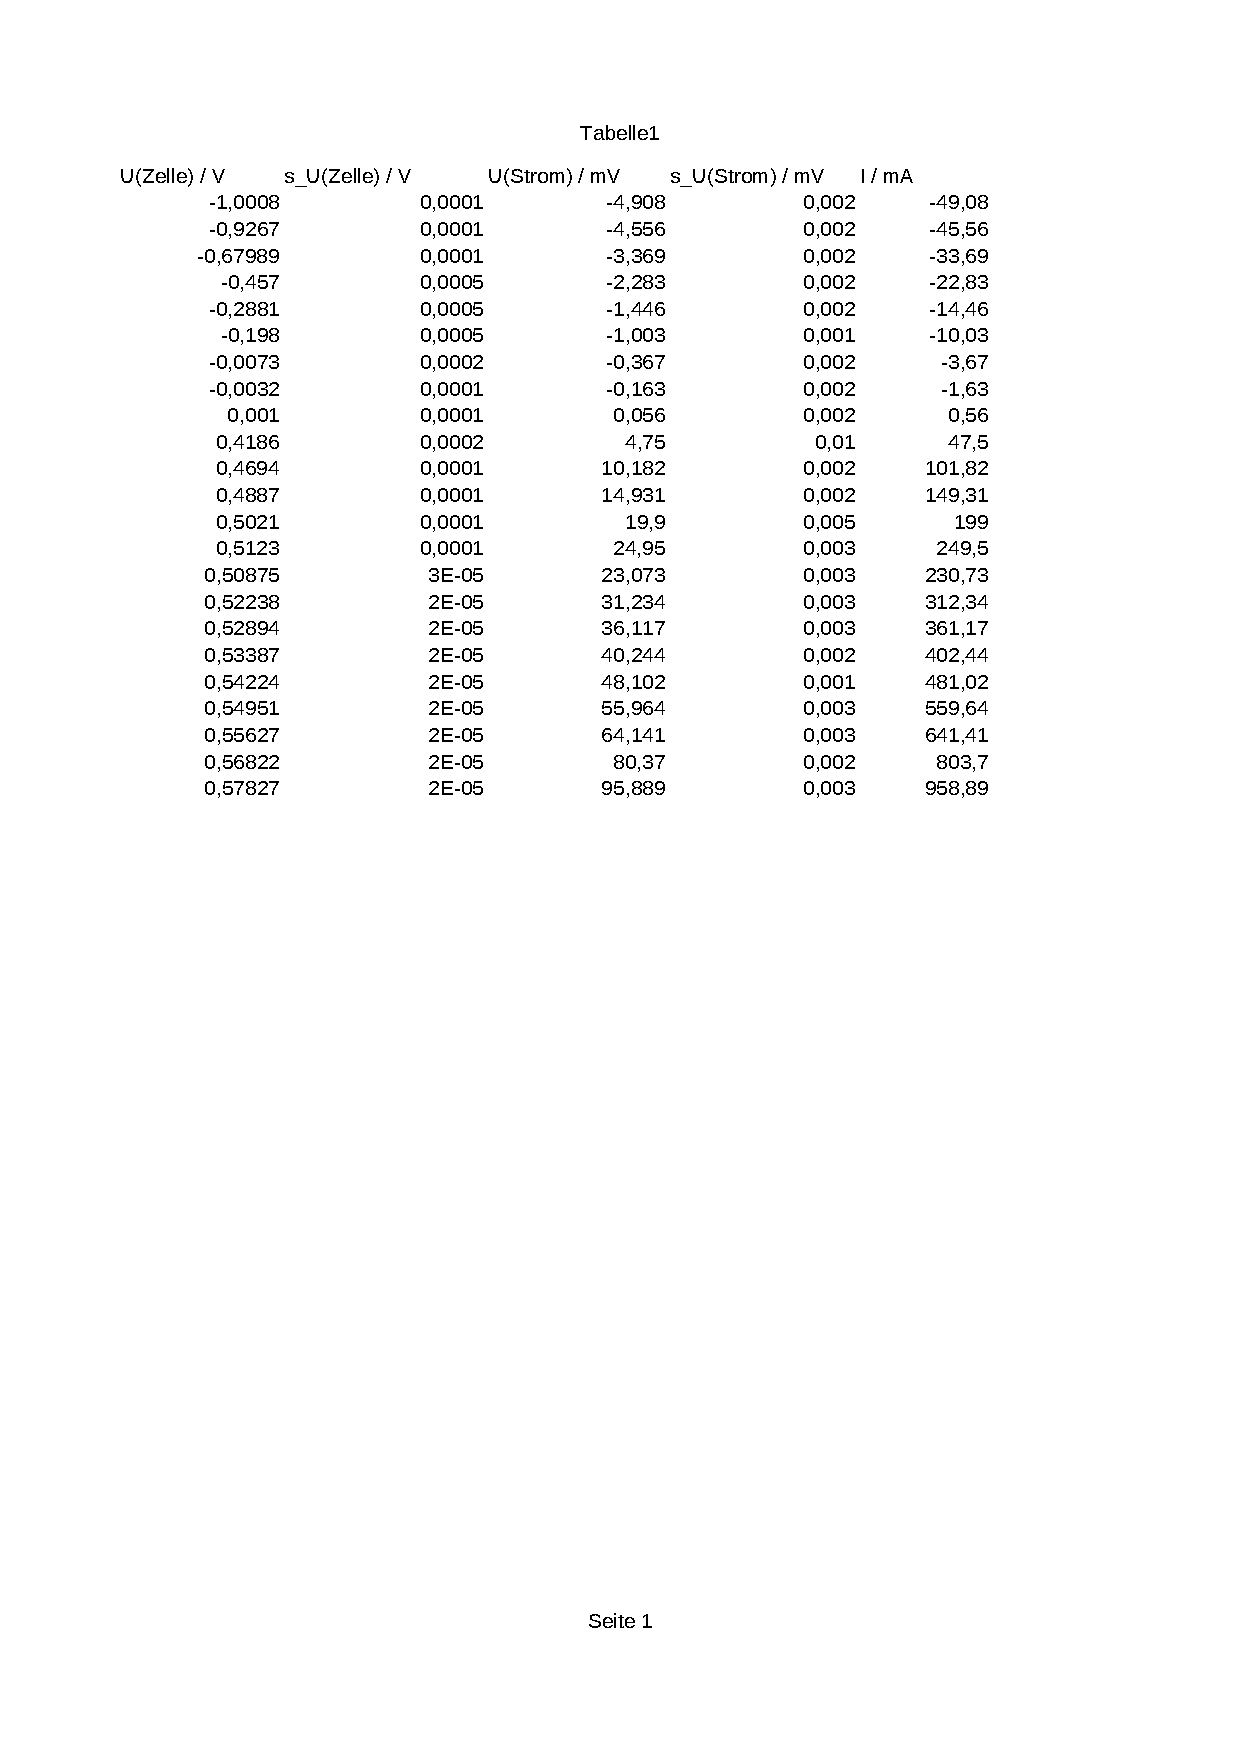
\includepdf[pages=-]{Messwerte/Messung33SiMonodunkel.pdf}
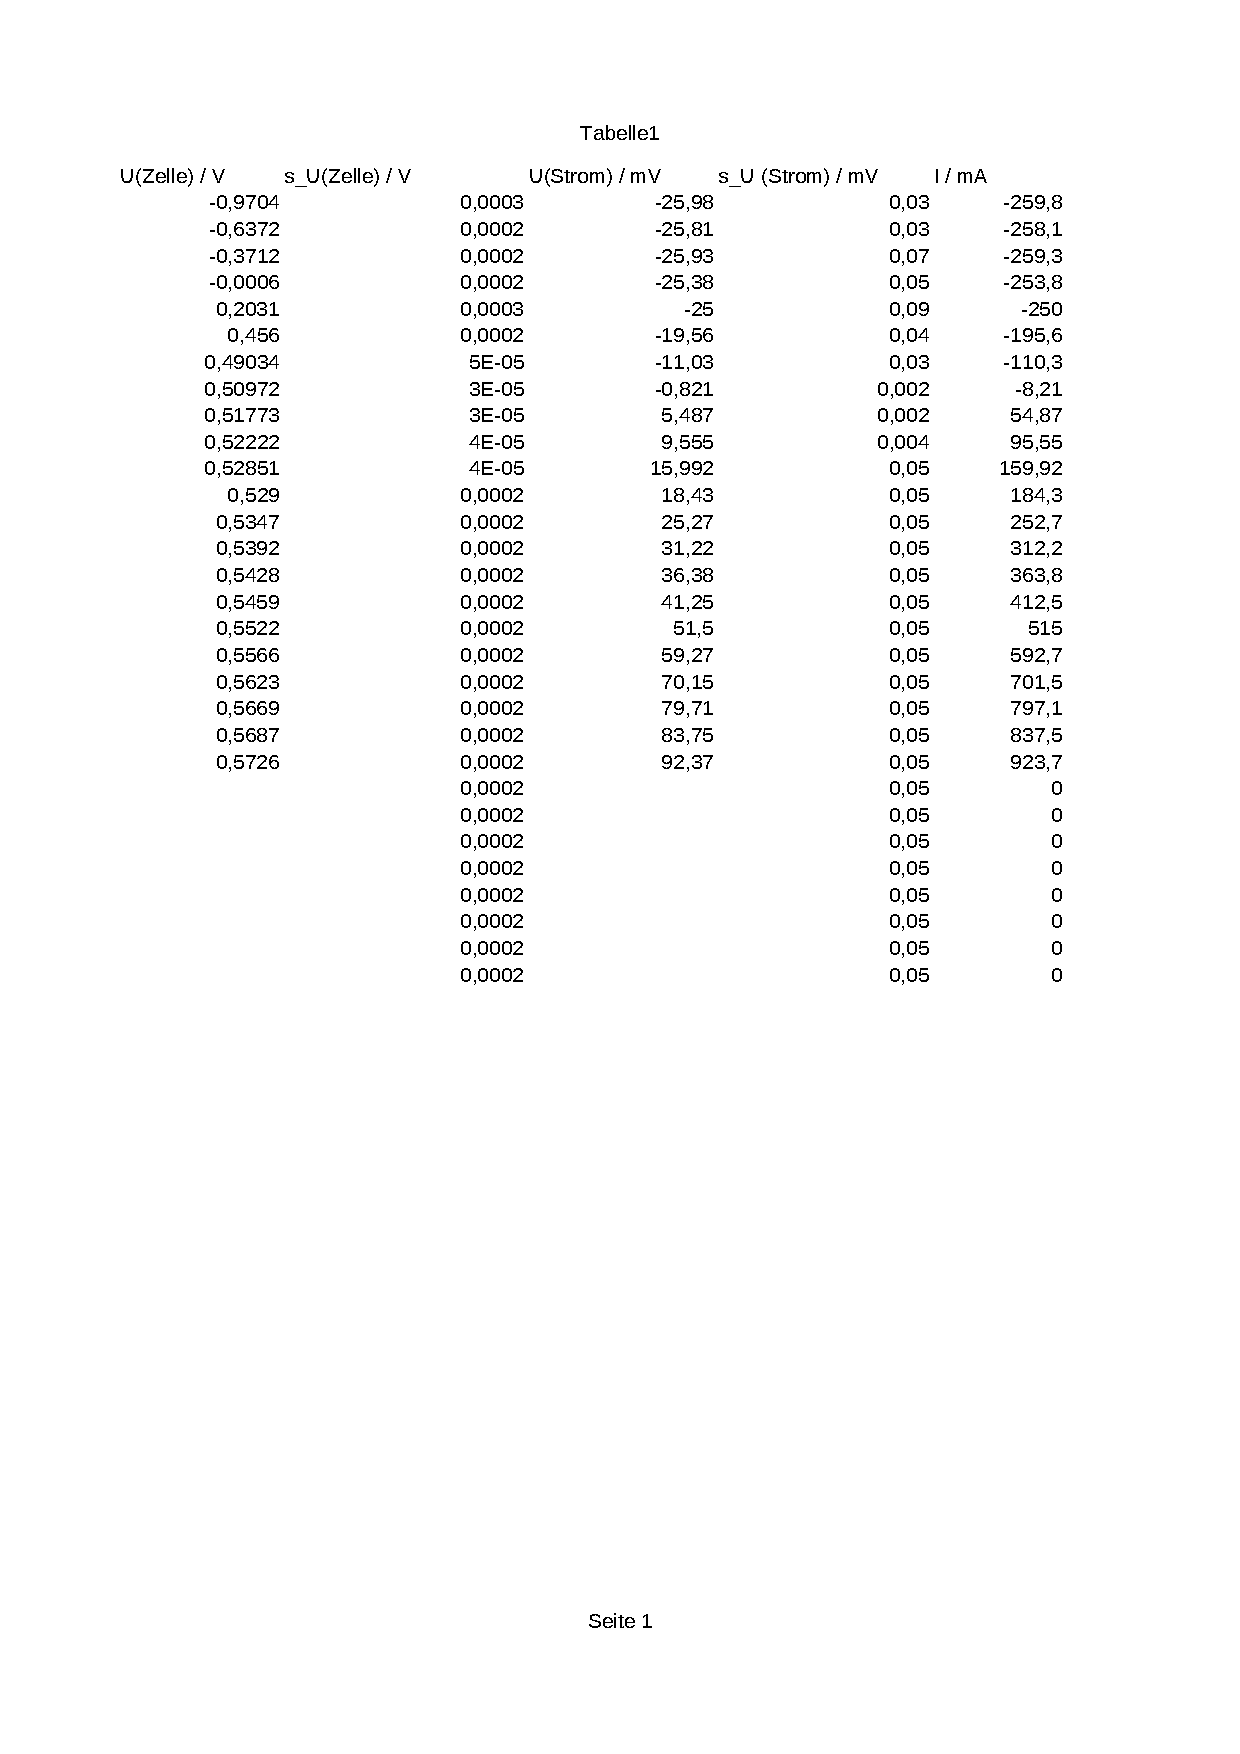
\includepdf[pages=-]{Messwerte/Messung33SiMulti130.pdf}
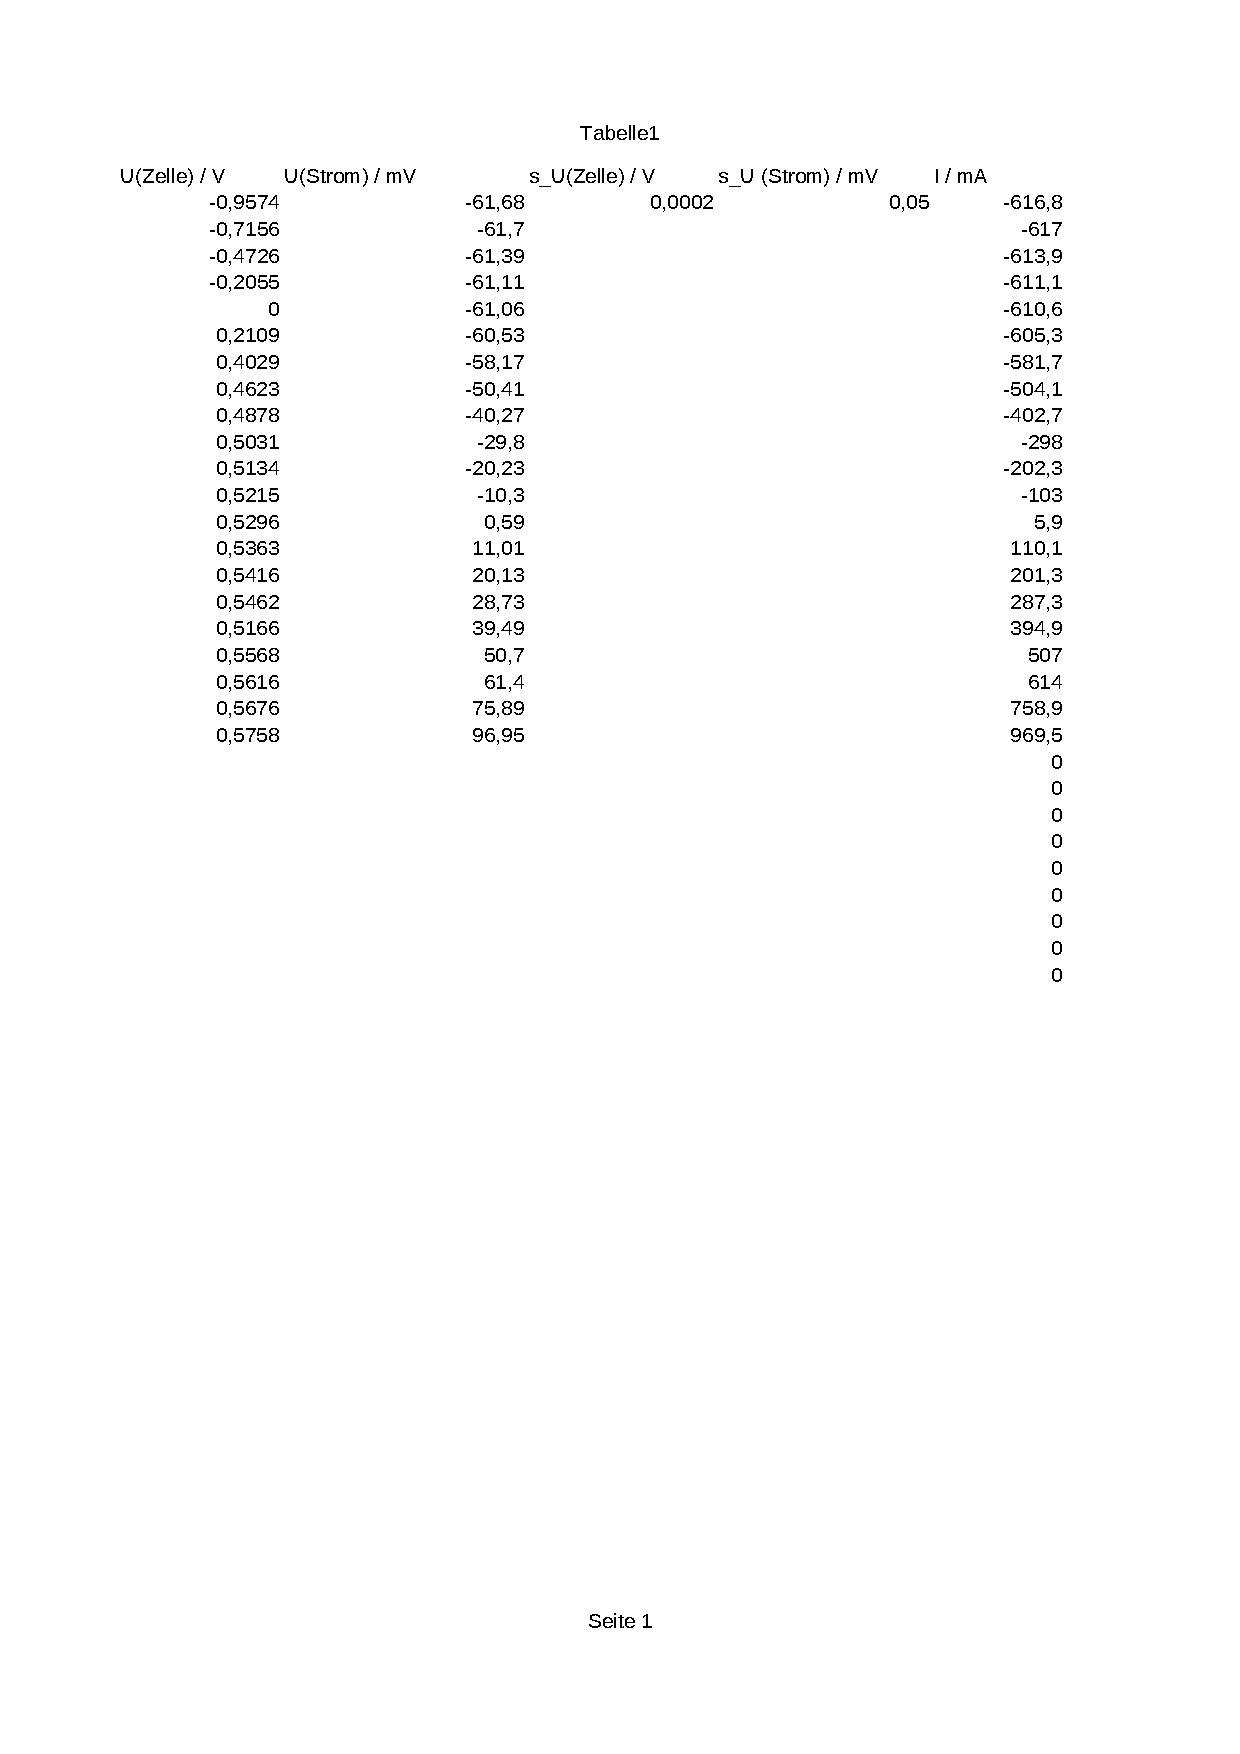
\includepdf[pages=-]{Messwerte/Messung33SiMulti180.pdf}
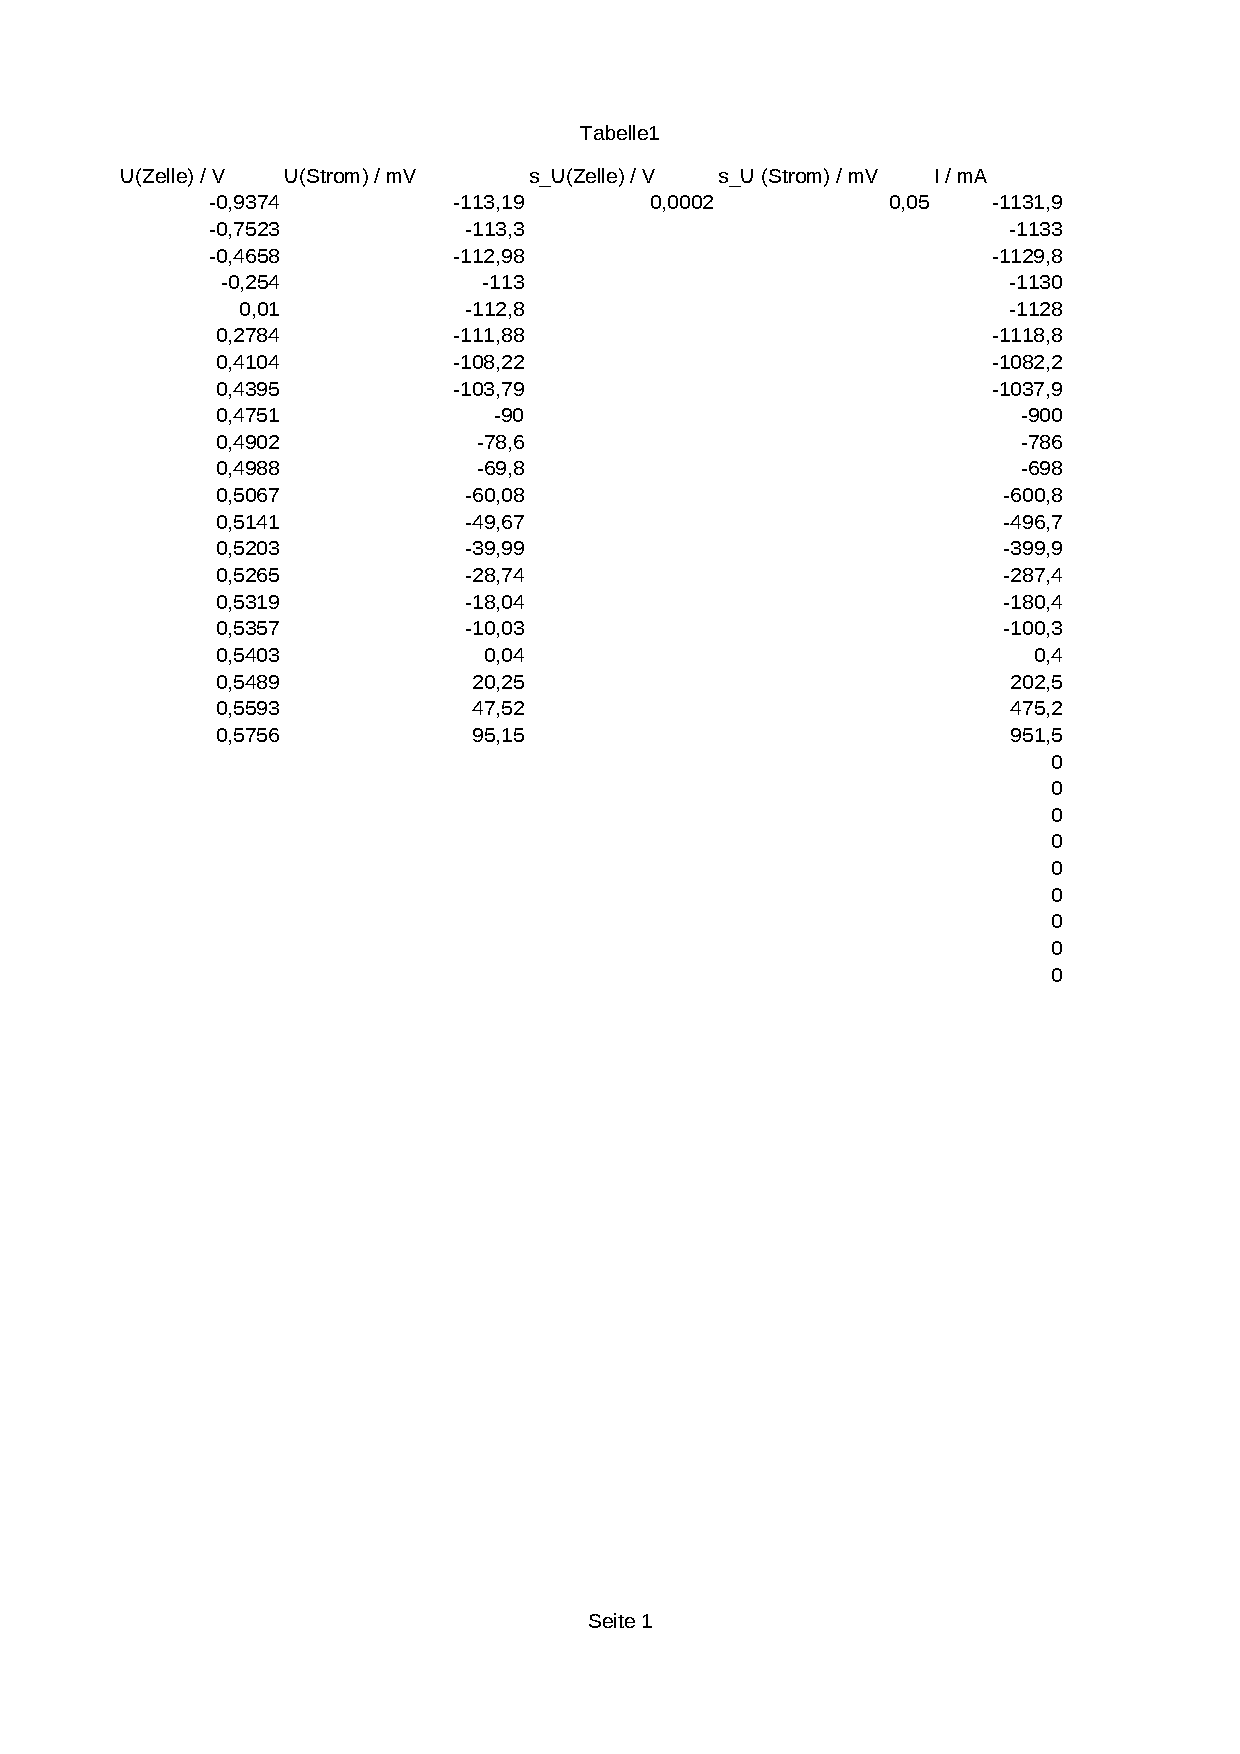
\includepdf[pages=-]{Messwerte/Messung33SiMulti230.pdf}
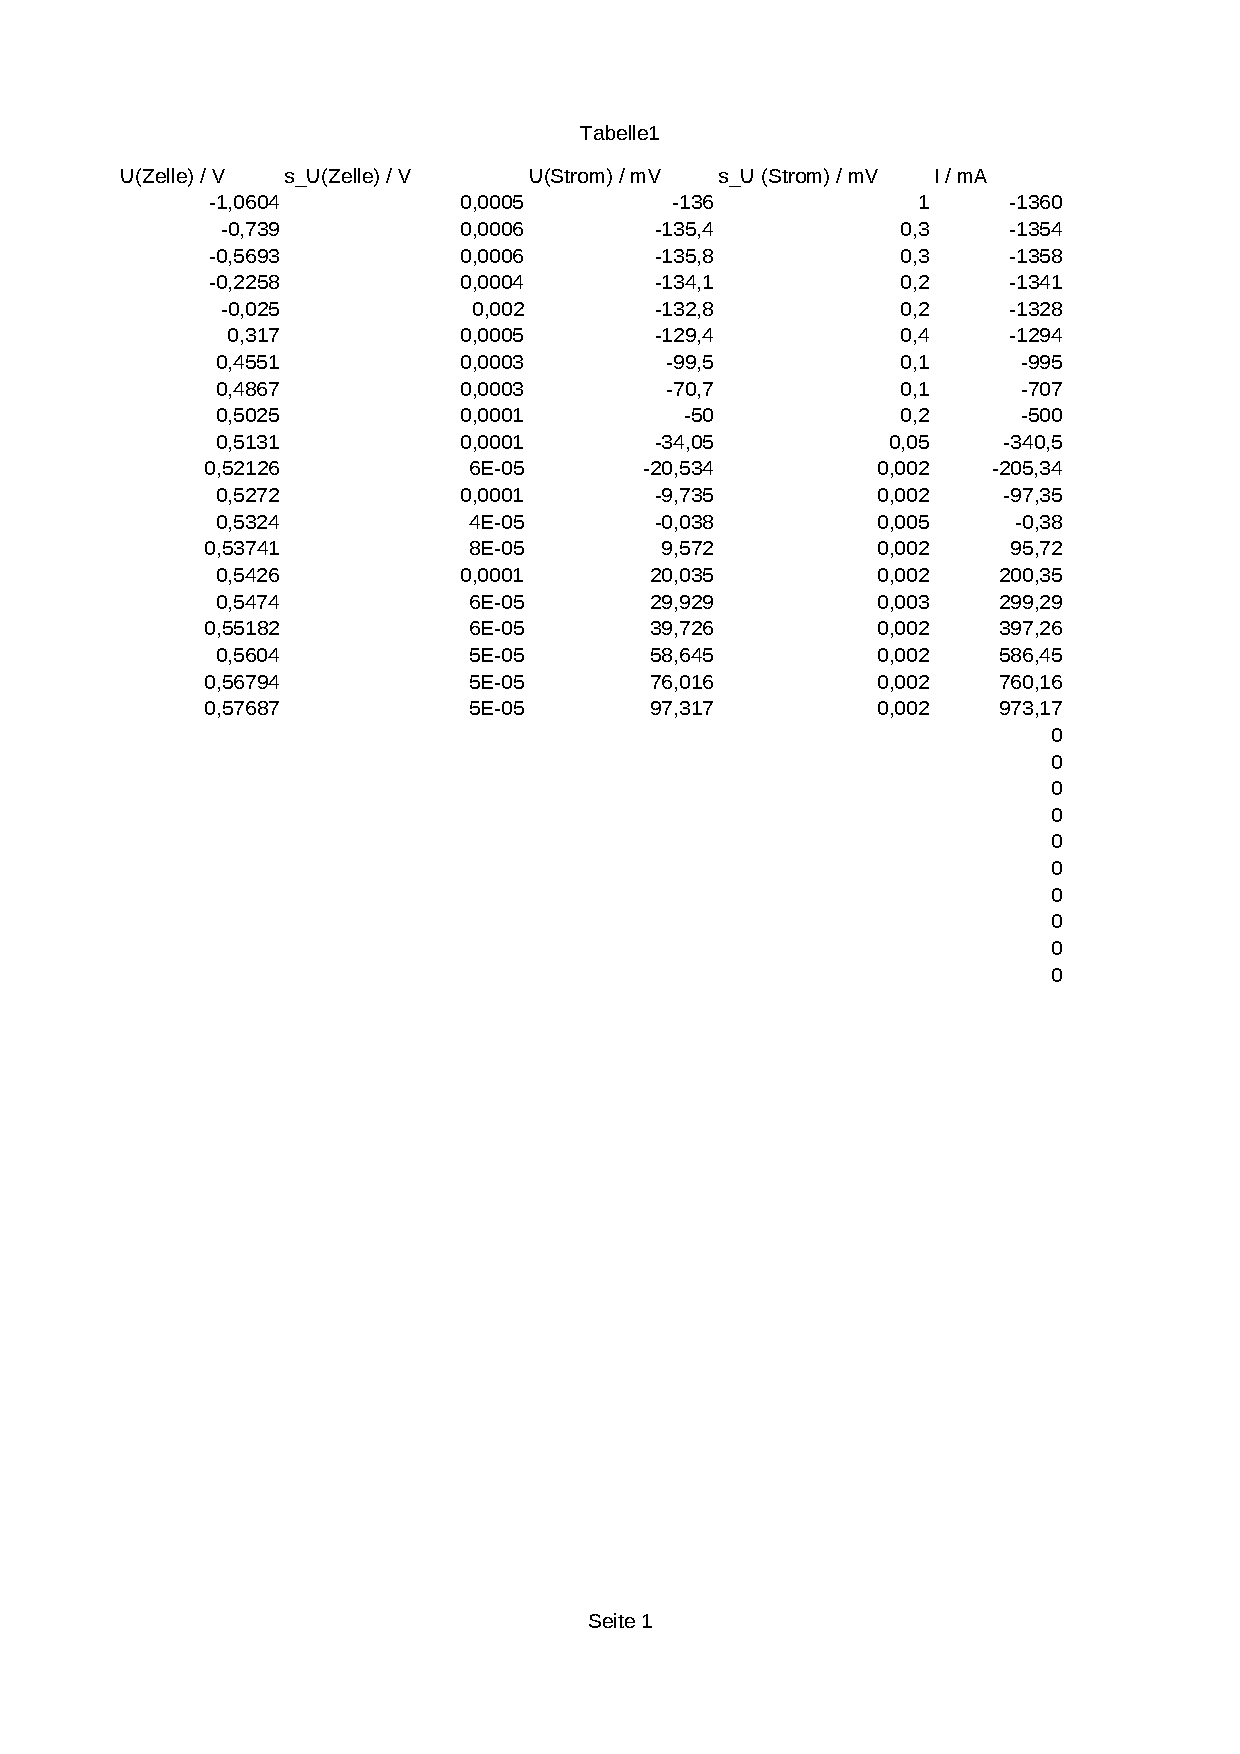
\includepdf[pages=-]{Messwerte/Messung33SiMono230.pdf}

\clearpage
\section{Fitten der Shockley-Gleichung}

\begin{figure}[ht]
    \centering
    \includegraphics[width = \linewidth]{Bilder/SiMonoDunkelPlot.pdf}
    \caption{Gefittete Schockley-Gleichung an das Mono-Si-Modul bei 130V}
\end{figure}
\begin{figure}[ht]
    \centering
    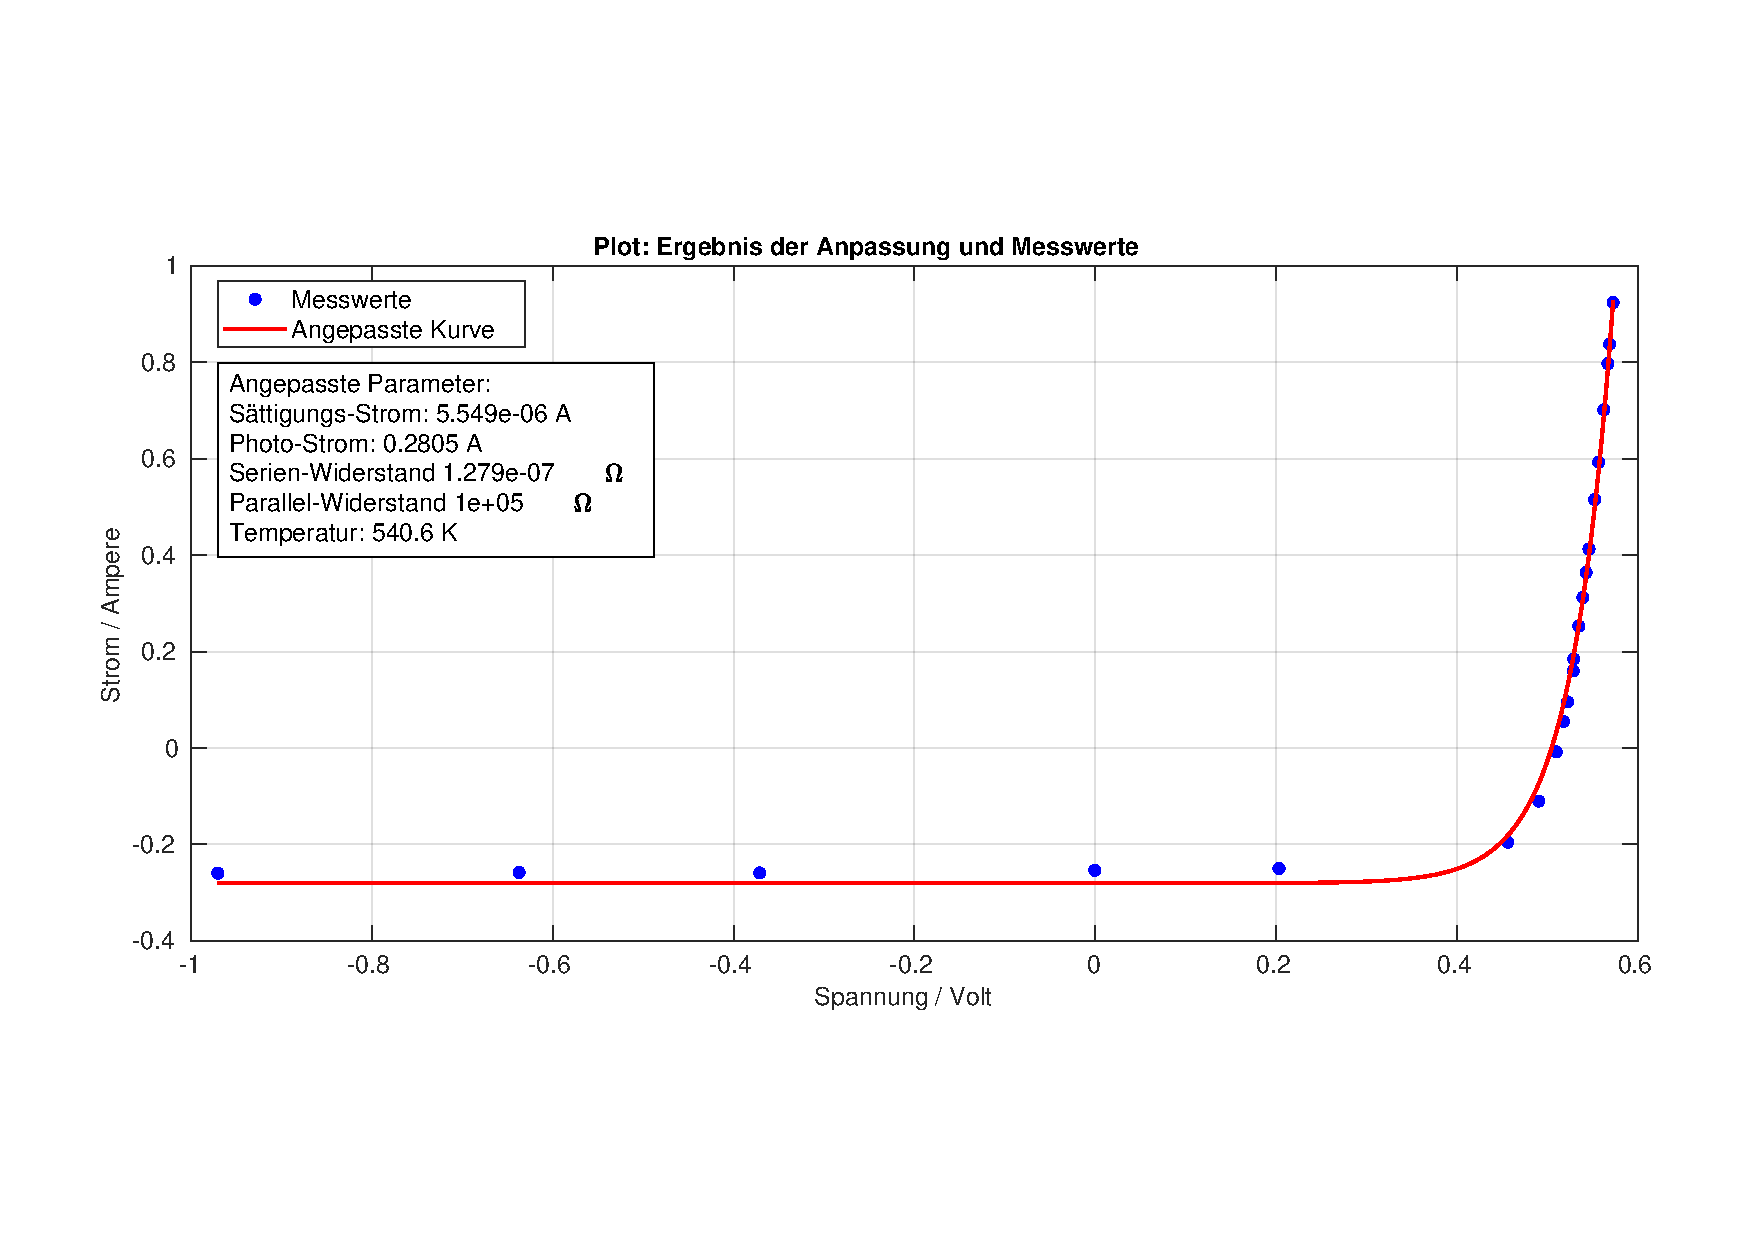
\includegraphics[width = \linewidth]{Bilder/SiMulti130Plot.pdf}
    \caption{Gefittete Schockley-Gleichung an das Mono-Si-Modul bei 130V}
\end{figure}
\begin{figure}[ht]
    \centering
    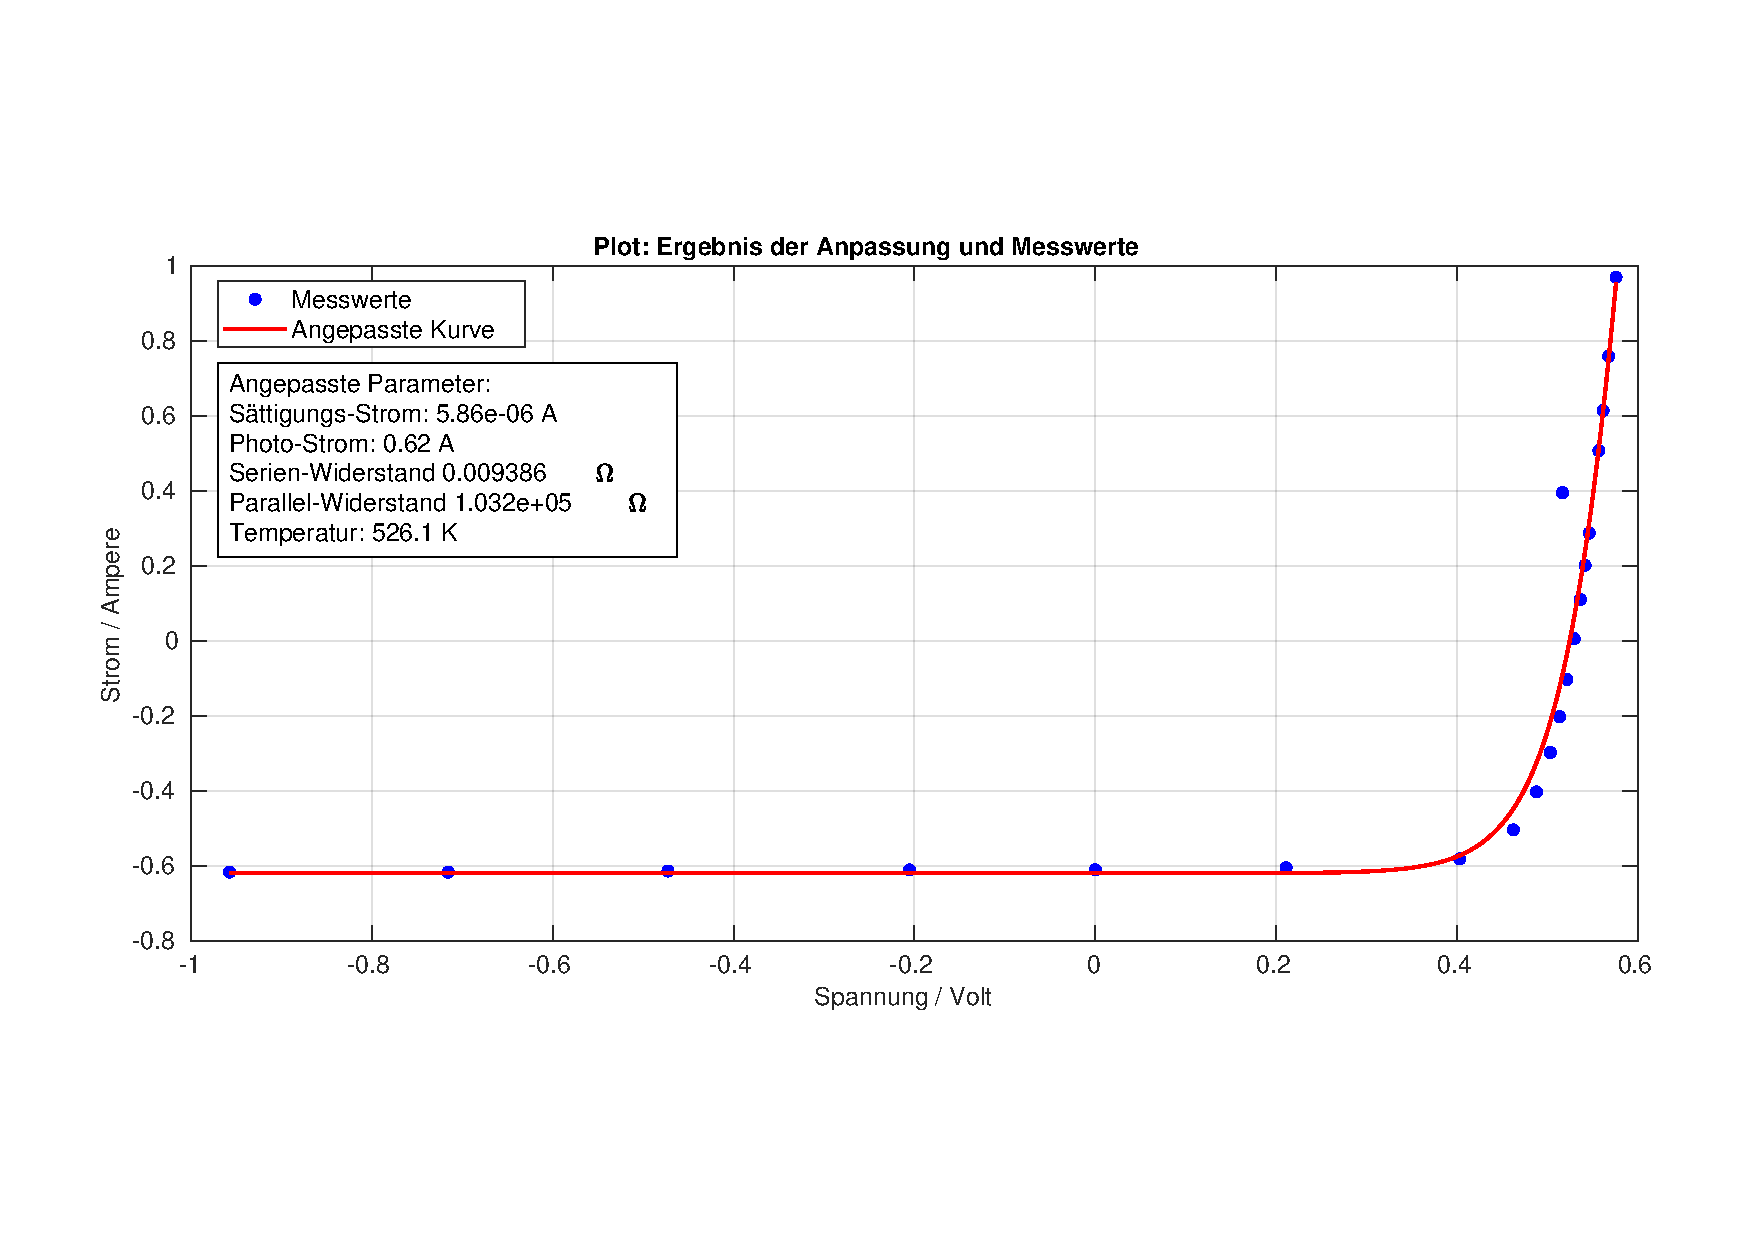
\includegraphics[width = \linewidth]{Bilder/SiMulti180Plot.pdf}
    \caption{Gefittete Schockley-Gleichung an das Mono-Si-Modul bei 130V}
\end{figure}
\begin{figure}[ht]
    \centering
    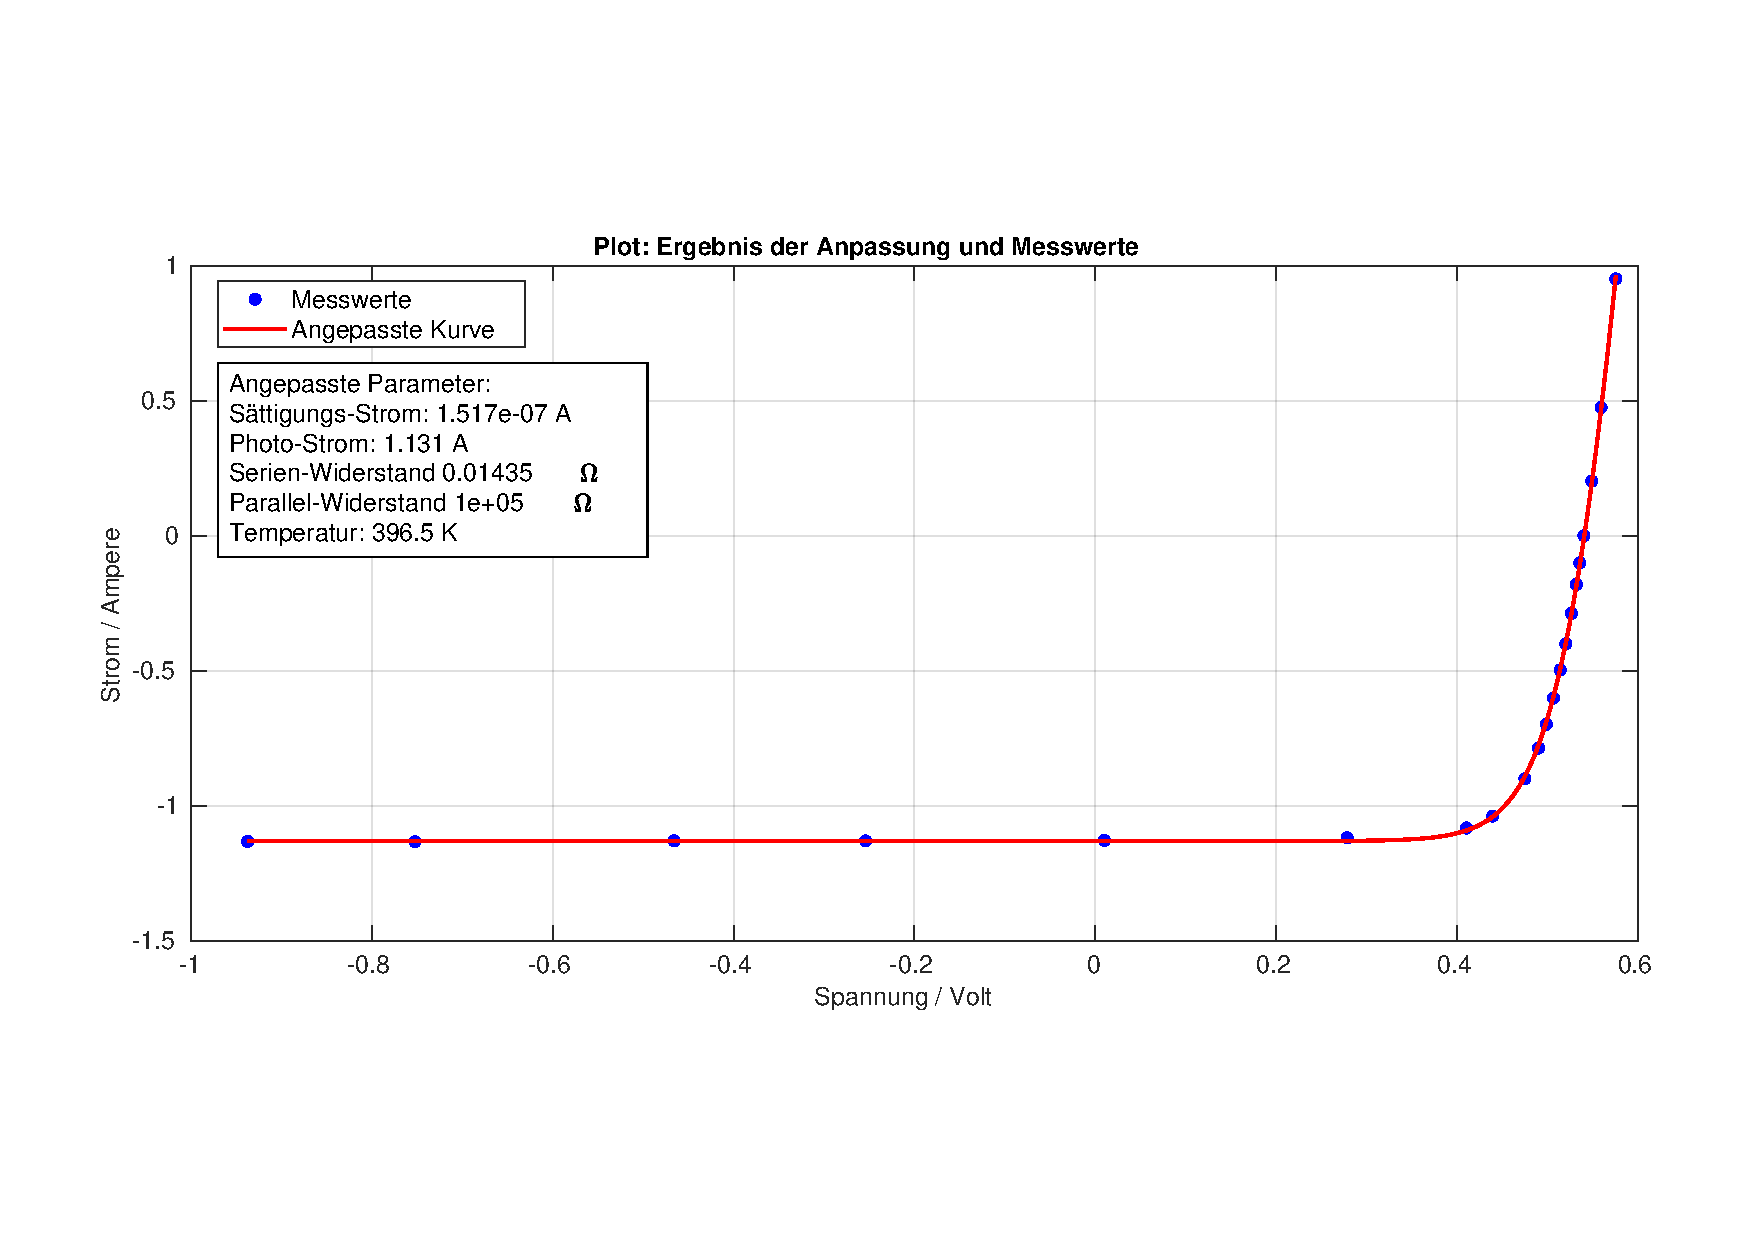
\includegraphics[width = \linewidth]{Bilder/SiMulti230Plot.pdf}
    \caption{Gefittete Schockley-Gleichung an das Mono-Si-Modul bei 130V}
\end{figure}
\begin{figure}[ht]
    \centering
    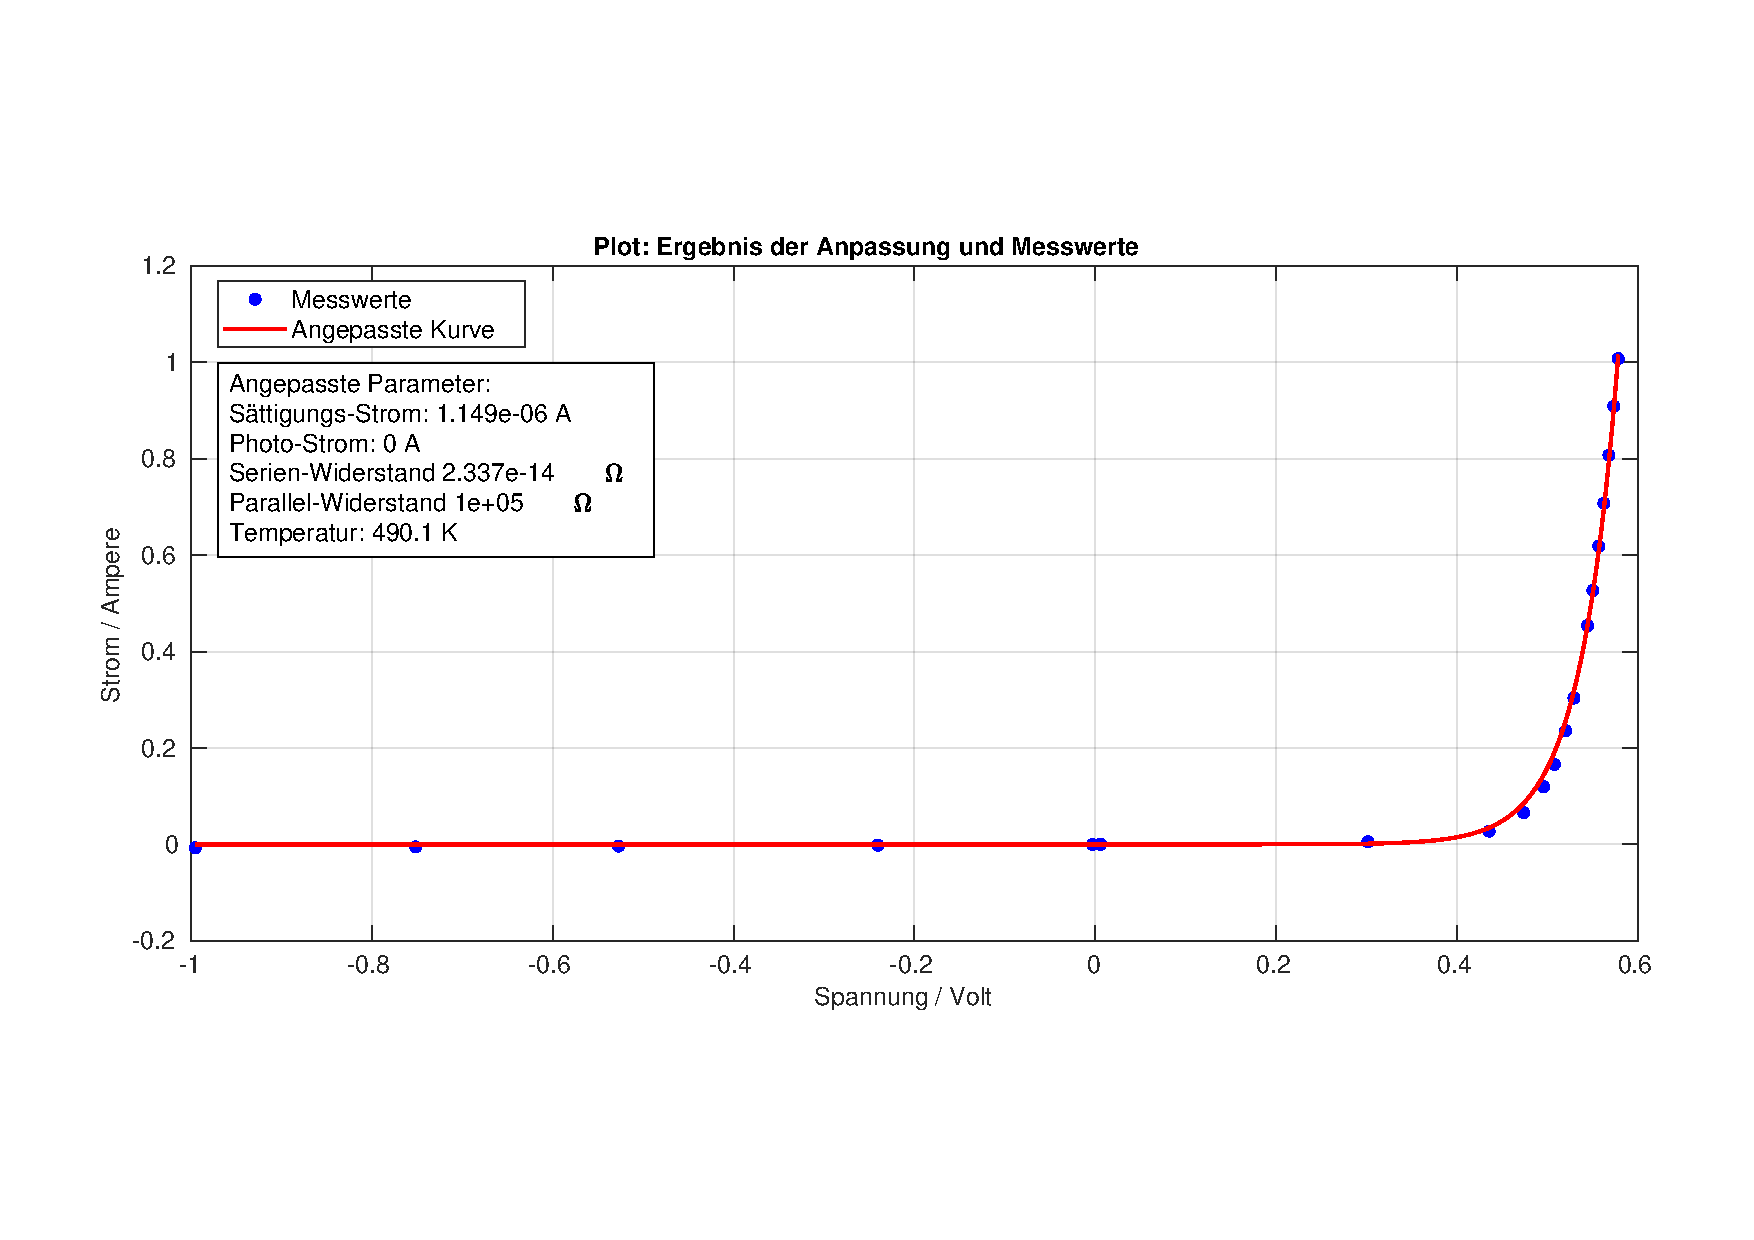
\includegraphics[width = \linewidth]{Bilder/SiMultiDunkelPlot.pdf}
    \caption{Gefittete Schockley-Gleichung an das Mono-Si-Modul bei 130V}
\end{figure}
\clearpage

\section{Wirkungsgrad}
\label{section:AnhangWirkungsgrad}

\begin{figure}[ht]
    \centering
    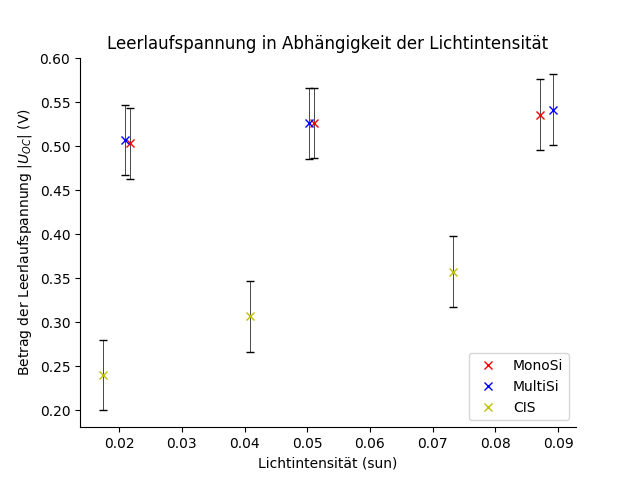
\includegraphics[width = \linewidth]{Bilder/PlotLeerlaufspannugnInt.png}
    \caption{Leerlaufspannung in Abhängigkeit der Lichtintensität}
\end{figure}

\begin{figure}[ht]
    \centering
    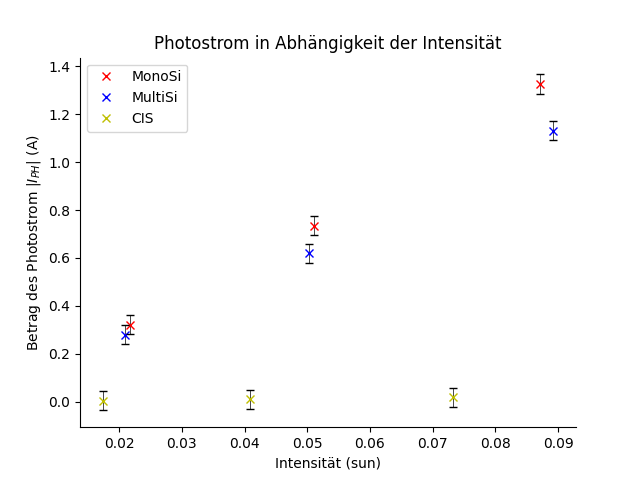
\includegraphics[width = \linewidth]{Bilder/PlotPhotostromInt.png}
    \caption{Photostrom in Abhängigkeit der Lichtintensität}

\end{figure}

\begin{figure}[ht]
    \centering
    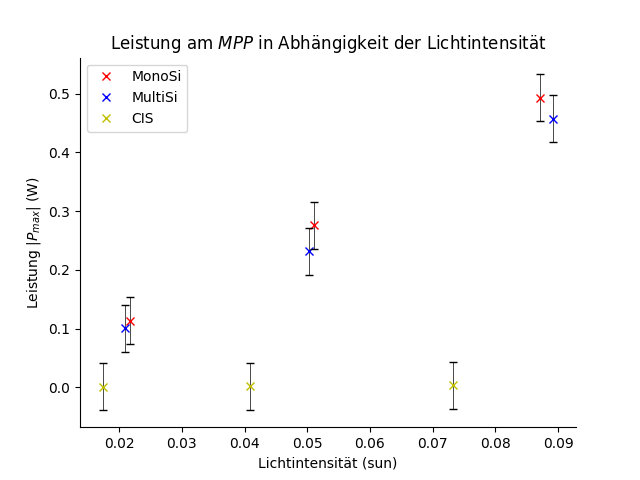
\includegraphics[width = \linewidth]{Bilder/PlotPMAXInt.png}
    \caption{Maximale Leistung $P_{Max}$ in Abhängigkeit der Lichtintensität}  
\end{figure}

\begin{figure}[ht]
    \centering
    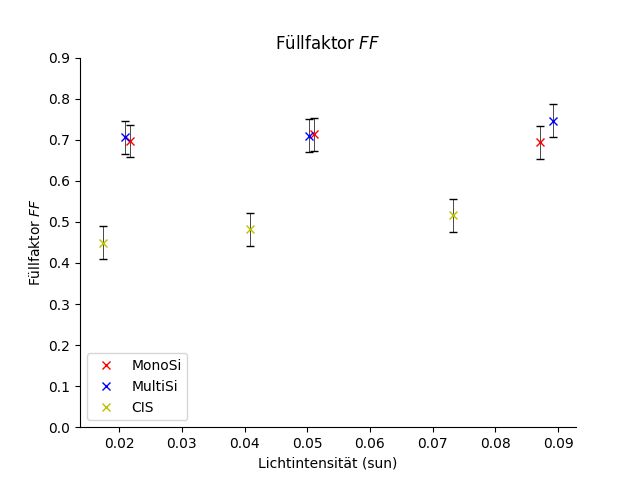
\includegraphics[width = \linewidth]{Bilder/PlotFFInt.png}
    \caption{Füllfaktor $FF$ in Abhängigkeit der Lichtintensität}  
\end{figure}
